
\subsection{Task Suite}

% Table of tasks
\begin{table}[htbp]
\centering
\caption{Audit task suite and reward environments.}
\label{tab:tasks}
\begin{tabular}{llll}
\toprule
\textbf{Task} & \textbf{Method} & \textbf{Reward} & \textbf{Dataset} \\
\midrule
Math RL (Arithmetic) & GRPO & Binary correctness & Generated \\
Math RL (GSM8K) & GRPO & Binary correctness & GSM8K \\
Chat SFT & SFT & Cross-entropy loss & NoRobots \\
Preference (Shorter) & DPO & Pairwise preference & Generated \\
Distillation (Off-Policy) & SFT & KL divergence & OpenThoughts3 \\
Distillation (On-Policy) & IS Loss & $\log p_t - \log p_s$ & Online \\
\bottomrule
\end{tabular}
\end{table}

\subsection{Cross-Library Implementation}

% Table of implementations
\begin{table}[htbp]
\centering
\caption{Implementations across RL libraries.}
\label{tab:implementations}
\begin{tabular}{lll}
\toprule
\textbf{Library} & \textbf{Implementation} & \textbf{Category} \\
\midrule
TRL (HuggingFace) & GRPOTrainer, DPOTrainer, SFTTrainer & LLM-native \\
Stable Baselines3 & PPO & Classic RL \\
CleanRL & PPO (single-file) & Research RL \\
Tianshou & PPO & Modular RL \\
PufferLib & PPO (high-throughput) & High-perf RL \\
rl\_games (NVIDIA) & PPO (GPU-optimized) & High-perf RL \\
d3rlpy & CQL (offline) & Offline RL \\
\bottomrule
\end{tabular}
\end{table}

\subsection{Hyperparameter Mapping}

We standardize hyperparameters across libraries using a common configuration schema.
Table~\ref{tab:hyperparams} shows the mapping from Tinker PPO defaults to each library's
native parameter names.

\begin{table}[htbp]
\centering
\caption{Hyperparameter mapping across libraries (PPO defaults).}
\label{tab:hyperparams}
\begin{tabular}{lcccccc}
\toprule
\textbf{Parameter} & \textbf{TRL} & \textbf{SB3} & \textbf{CleanRL} & \textbf{Tianshou} & \textbf{PufferLib} & \textbf{rl\_games} \\
\midrule
Learning rate & $10^{-4}$ & $10^{-4}$ & $10^{-4}$ & $10^{-4}$ & $10^{-4}$ & $10^{-4}$ \\
Clip range ($\epsilon$) & 0.2 & 0.2 & 0.2 & 0.2 & 0.2 & 0.2 \\
Entropy coeff. & 0.01 & 0.01 & 0.01 & 0.01 & 0.01 & 0.01 \\
GAE $\lambda$ & 0.95 & 0.95 & 0.95 & 0.95 & 0.95 & 0.95 \\
Discount $\gamma$ & 0.99 & 0.99 & 0.99 & 0.99 & 0.99 & 0.99 \\
Max grad norm & 0.5 & 0.5 & 0.5 & 0.5 & 0.5 & 0.5 \\
Target KL & 0.01 & 0.01 & 0.01 & N/A & N/A & N/A \\
\bottomrule
\end{tabular}
\end{table}

\subsection{Reward Verification}

% Figure 3: Verifiable Reward Flow
\begin{figure}[t]
\centering
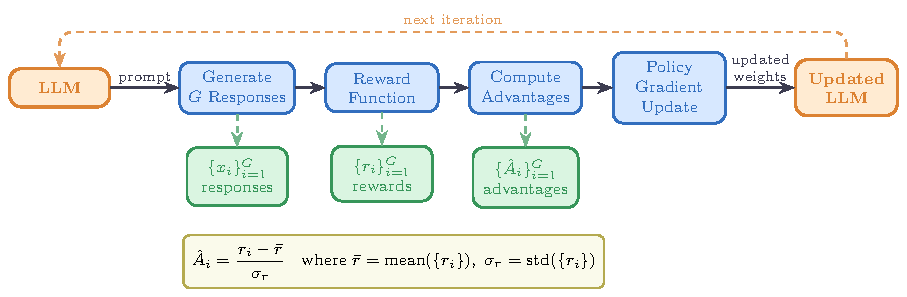
\includegraphics[width=0.55\textwidth]{tikz/reward_flow.pdf}
\caption{Verifiable reward paradigm in \ours{}. Unlike learned reward models,
verifiable rewards reduce reliance on reward models, but they can still induce
reward hacking through parser artifacts, format shortcuts, length effects, and
train-prompt overfitting. Verifiable rewards do not eliminate reward hacking.}
\label{fig:reward-flow}
\end{figure}

\subsection{Baselines: Floor and Ceiling}

Borrowing hygiene from benchmark design~\cite{agarwal2021deep}, we establish
clear performance bounds for the arithmetic sanity task:

\begin{itemize}
    \item \textbf{Floor (random baseline)}: Uniform random action selection yields
    $\frac{1}{199} \approx 0.50\%$ accuracy on the arithmetic task.
    \item \textbf{Ceiling (oracle)}: Direct computation achieves $100\%$ accuracy.
    \item \textbf{Human baseline}: College-level adults achieve $\sim$99.5\% on
    two-digit addition under timed conditions.
\end{itemize}

\begin{table}[htbp]
\centering
\caption{Evidence types and permitted interpretations in this audit.}
\label{tab:evidence_types}
\small
\begin{tabular}{@{}p{0.30\linewidth}p{0.58\linewidth}@{}}
\toprule
\textbf{Evidence type} & \textbf{Supports}\\
\midrule
Online training reward & Optimization dynamics under the rollout reward parser.\\
Held-out GSM8K & Capability/generalization claims for the evaluated slice.\\
Tool-use JSON reward & Schema-format behavior; not executed tool success.\\
HumanEval/MATH probes & Reward-environment behavior under limited harnesses.\\
PPO/GRPO rows & Stack sensitivity and reporting hygiene; not algorithm ranking.\\
\bottomrule
\end{tabular}
\end{table}

% =============================================================================
\section{Experimental Setup}
\label{sec:setup}
% =============================================================================

\subsection{Models}

We evaluate a total of 32+ models spanning \textbf{0.6B to 671B parameters
across 5 model families}, organized into three tiers by compute scale:

\paragraph{Small scale (0.6B--8B).}
Qwen3-0.6B-Instruct, Qwen3.5-4B, Qwen3-4B, Qwen3-8B,
Llama-3.2-1B, Llama-3.2-3B, Llama-3.1-8B-Instruct.

\paragraph{Mid scale (14B--32B).}
Qwen3-14B, Qwen3-30B-A3B (MoE), Qwen3-32B, Qwen3.5-27B,
GPT-OSS-20b, Kimi-K2 (selected scale points).

\paragraph{Larger-model support probes (70B--671B).}
Qwen3-235B-A22B (MoE), DeepSeek-V3.1 ($\approx$671B total / 37B active),
Nemotron-120B, and selected 397B-class MoE architectures.
Larger-model probes are evaluated via the Tinker API in inference mode
with standardized generation parameters; LoRA fine-tuning at this
scale is conducted on selected checkpoints (see Section~\ref{sec:frontier}).

\paragraph{Model family coverage.}
The audit corpus covers (1) \textbf{Qwen3}: a dense family from 0.6B to 32B;
(2) \textbf{Qwen3.5}: an improved series including 4B and 27B;
(3) \textbf{Llama-3.x}: Meta's 1B--8B instruction-tuned models;
(4) \textbf{DeepSeek-V3.1}: a frontier MoE optimized for reasoning;
(5) \textbf{Nemotron-120B}: NVIDIA's dense frontier model;
and emerging architectures \textbf{GPT-OSS-20b} and \textbf{Kimi-K2}.

\subsection{Training Protocol}

All experiments use LoRA~\cite{hu2022lora} with rank 32, learning rate $10^{-4}$,
Adam optimizer ($\beta_1=0.9$, $\beta_2=0.95$, $\epsilon=10^{-8}$).

\paragraph{Seed management.} Only selected TRL baselines and the GSM8K
held-out evaluation use five seeds; the majority of Tinker runs are
single-seed.  When seeds are set, we use
$\{42, 123, 456, 789, 1024\}$ for Python \texttt{random},
NumPy, PyTorch, and CUDA backends.

% Figure 4: Experiment Pipeline
\begin{figure}[t]
\centering
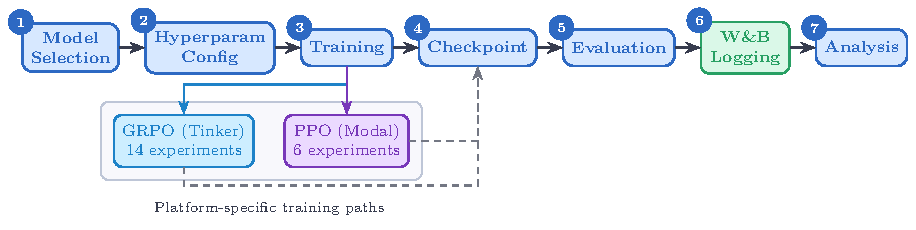
\includegraphics[width=\textwidth]{tikz/pipeline.pdf}
\caption{Experiment workflow pipeline.  Only selected TRL baselines and the
GSM8K held-out evaluation are run with five seeds; most Tinker runs are
single-seed.  Seeds feed centralized seed management, which forks into
metrics analysis and checkpoint storage before figure generation.}
\label{fig:pipeline}
\end{figure}

\subsection{Statistical Methodology}
\label{sec:statistical-policy}
Training steps within a run are autocorrelated and may be nonstationary. We
retain fixed-window summaries and descriptive coefficients, not step-iid
bootstrap intervals, first-versus-last-window tests, significance stars, or
claims that a multiplicity correction calibrates invalid p-values. Resampling
two arms independently is an unpaired bootstrap. Independence between runs does
not imply independence between steps. A block bootstrap would require a justified
dependence model and is not automatically reliable for a short evolving trace.

Seed/run-level inference requires actual independent observations, an identified
estimand, and an eligible matched comparison. Reconstructed vectors from a mean
and standard error cannot support an empirical seed bootstrap. Trustworthy mean,
SD, and sample count could support an analytic summary-statistic Welch test,
but only after task and cohort identity are resolved. An all-zero trace has
zero pooled variance: Cohen's $d=0/0$ is \emph{not estimable}, not zero with a
zero-width interval. One seed cannot estimate across-seed uncertainty; this does
not preclude separately justified conditional prompt-level inference.

\paragraph{Multiplicity and eligibility.}
The historical five-test, 20-test BH, and 38-test Bonferroni families were not
consistent. Primary hypotheses were not preregistered. We withdraw their
significance decisions rather than choosing a smaller denominator. Before any
future inference, a single versioned comparison registry must specify comparison
ID, cohort IDs, independent unit, estimand, eligibility, family ID, raw p-value,
adjustment, and adjusted p-value. Retrospective enumeration must be labeled as
such; missing comparisons do not silently reduce a prespecified family.
For example, the historical $t(4)=7.44$ gives a two-sided $p\simeq0.001743$ and
$38p\simeq0.06623$, not a family-wide significant result. This arithmetic check
does not establish that the underlying comparison is scientifically eligible.

\paragraph{Power illustration, not evidence.}
\texttt{TTestIndPower} uses a pooled equal-variance model, not Welch's degrees
of freedom. For five observations per arm, the equal-variance 80\%-power MDE
at unadjusted $\alpha=0.05$ is approximately $d=2.024$; using $0.05/5$ or
$0.05/38$ gives approximately $2.744$ or $3.778$. These are planning
illustrations, not observed-effect ``achieved power,'' not an endorsement of
any historical correction family, and not evidence for a measured effect.

\paragraph{Historical seed summaries.}
The TRL Qwen2.5-0.5B reference is labeled GSM8K in its baseline description
and arithmetic elsewhere. Task identity remains unresolved. Its reported
five-seed mean $0.734$ and SD $0.0703$ are retained as historical summaries
only; neither task label is selected as authoritative, and no reconstructed
seed bootstrap or cross-task comparison is asserted. The later five-seed
Qwen3-8B comparison against a fixed base is separate from the reviewed record.


\subsection{Compute Resources}

Experiments are distributed across two compute platforms:

\paragraph{Tinker API (14 experiments).}
Reward-probe experiments across Qwen3-8B, Qwen3-32B, Qwen3.5-4B, Qwen3.5-27B,
and Llama-3.1-8B-Instruct; larger-model evaluation on Qwen3-235B-A22B,
DeepSeek-V3.1, and Nemotron-120B; dense/MoE initialization probes; cross-task
tool-use experiments; and emerging architecture evaluation (GPT-OSS-20b,
Kimi-K2). Tinker provides scalable API access that makes larger-model
reward probes economically tractable.

\paragraph{Modal H100 GPU cluster (6 experiments).}
PPO baseline training on Qwen3-8B and Llama-3.1-8B; full HumanEval
proxy benchmark evaluation; KL divergence tracking across GRPO training steps;
and held-out evaluation for Qwen3-32B and Qwen3.5-27B. Modal H100s
provide the low-level GPU access required for PPO value-model training.

All experiment logs are available on Weights \& Biases (project:
\texttt{tinker-rl-lab-world-class}) and model checkpoints on HuggingFace
Hub (\url{https://huggingface.co/arvindcr4/tinker-rl-bench-*}).
See Appendix~\ref{app:compute} for full details. Total project compute:
$\sim$1,200 A100 GPU-hours across both platforms.

% =============================================================================
\section{Results}
\label{sec:results}
% =============================================================================

\paragraph{Metric taxonomy.}
All results below use one of three non-interchangeable quantities.  \textbf{Online
training reward} is the scalar reward observed during training on the sampled
training prompts or task episodes; for GSM8K it is a binary boxed-answer reward,
but it is still an online training statistic rather than a held-out benchmark.
\textbf{Held-out accuracy} is reported only when a checkpoint is evaluated after
training on a disjoint evaluation split or fixed held-out slice with a stated
sample size and confidence interval.  \textbf{Proxy diagnostics} such as
zero-variance fraction (ZVF), stability index (SI), peak-to-tail drift (PTD),
and surrogate-loss traces are telemetry-derived signals about optimization or
policy stability; they are not accuracy numbers and are not treated as reward
improvements.  Tables and figures are labelled by metric family, and we do not
rank models by mixing these families.



\subsection{Online GSM8K Training Rewards}
\label{sec:main_results}

This paper is an empirical audit of a heterogeneous run corpus, not a controlled
algorithm benchmark. Most Tinker runs are single-seed, short-horizon, and
evaluated by online training reward. We therefore use them to study reward
dynamics, failure modes, and stack sensitivity. Capability claims are restricted
to evaluations with held-out prompts and explicit base-model controls; under that
standard, the GSM8K lift is small and non-significant. Table~\ref{tab:evidence_types}
summarizes the evidence hierarchy used throughout the paper.

\begin{table}[htbp]
\centering
\caption{Evidence types and permitted interpretations in this audit.}
\label{tab:evidence_types_detail}
\scriptsize
\begin{tabular}{p{3.2cm}p{3.0cm}p{2.5cm}p{2.5cm}}
\toprule
\textbf{Evidence type} & \textbf{Runs} & \textbf{Independent unit} & \textbf{Can support} \\
\midrule
Tinker GRPO traces & Mostly single-seed, 30-step & run/checkpoint & descriptive dynamics only \\
GSM8K held-out base-vs-GRPO & 5 reported seeds; item IDs unresolved & seed vs. fixed baseline & later evidence, not reviewed record \\
Top-checkpoint GSM8K audit & selected checkpoints & checkpoint & aggregate withdrawn; selection bias \\
ZVF validation & 22 deduplicated runs & run & triage claim only \\
Tool-use / HumanEval / MATH & proxy or harness-bound & task-specific trace & no broad capability claim \\
\midrule
\multicolumn{4}{p{11.2cm}}{\small \textit{Note:} Because many runs are single-seed and step-level rewards are autocorrelated within traces, we avoid treating per-step samples as independent experimental replicates. Inferential tests are reported only when the independent unit is a seed, prompt, or independently replicated run. Step-level reward samples inside a single training trace are treated as autocorrelated telemetry, not independent observations.} \\
\bottomrule
\end{tabular}
\end{table}

Table~\ref{tab:main_results} is the source-of-truth ledger for online GSM8K
training reward.  The reported columns are peak training reward and the mean
training reward over the final ten logged steps.  These values summarize
optimization behavior under each stack and seed; they are not held-out accuracy.
Partial experiments, where fewer steps than planned were completed, are marked
$\dagger$ and should be interpreted only as partial training traces.

\begin{table*}[t]
\centering
\caption{\textbf{Online GSM8K training reward ledger.} Peak training reward and
last-10-step mean training reward are reported separately from held-out
accuracy. All Tinker runs are single-seed; all Modal runs are single-seed on
H100. $\dagger$~Training interrupted; reported metrics are from available
steps.}
\label{tab:main_results}
\scriptsize
\setlength{\tabcolsep}{3pt}
\begin{tabular}{@{}l l l l r c c@{}}
\toprule
\textbf{Algo} & \textbf{Plat.} & \textbf{Model} & \textbf{Size} & \textbf{Steps} & \textbf{Peak train R} & \textbf{Last-10 train R} \\
\midrule
\multicolumn{7}{l}{\textit{GRPO on Tinker API (GSM8K training reward; not held-out accuracy)}} \\
\midrule
GRPO & Tinker & Qwen3-8B & 8B & 30 & 62.5\% & 34.4\% \\
GRPO & Tinker & Qwen3.5-4B & 4B & 30 & 100\% & 85.0\% \\
GRPO & Tinker & Qwen3.5-27B$^\dagger$ & 27B & 10 & 75.0\% & 43.7\% \\
GRPO & Tinker & Qwen3-32B$^\dagger$ & 32B & 10 & 31.2\% & 25.0\% \\
GRPO & Tinker & Llama-3.1-8B-Inst & 8B & 30 & 100\% & 84.4\% \\
GRPO & Tinker & DeepSeek-V3.1 & 671B (37B) & 20 & 100\% & 85.0\% \\
GRPO & Tinker & Nemotron-120B$^\dagger$ & 120B & 20 & 87.5\% & 16.2\% \\
GRPO & Tinker & Qwen3-235B-A22B$^\dagger$ & 235B (22B) & 15 & 100\% & 100\% \\
GRPO & Tinker & Q3-30B-A3B$^\dagger$ & 30B (3B) & partial & 50.0\% & 32.5\% \\
GRPO & Tinker & Q3-30B-Inst$^\dagger$ & 30B (3B) & partial & 100\% & 100\% \\
GRPO & Tinker & Kimi-K2 & MoE & 20 & 100\% & 62.5\% \\
\midrule
\multicolumn{7}{l}{\textit{Campaign Extension: Additional Runs Under the Training-Reward Parser (GRPO, Tinker)}} \\
\midrule
GRPO & Tinker & Qwen3-8B-Base & 8B & 30 & 100\% & 85.6\% \\
GRPO & Tinker & Kimi-K2-Thinking & MoE & 30 & 100\% & 95.8\% \\
GRPO & Tinker & Kimi-K2.5 & MoE & 30 & 100\% & 62.5\% \\
GRPO & Tinker & GPT-OSS-120B & 120B & 30 & 100\% & 87.5\% \\
GRPO & Tinker & Qwen3.5-397B & 397B (17B) & 30 & 100\% & 97.9\% \\
GRPO & Tinker & Llama-3.1-70B & 70B & 30 & 56.2\% & 36.4\% \\
GRPO & Tinker & DS-V3.1-Base & 671B (37B) & 30 & 81.2\% & 57.3\% \\
GRPO & Tinker & Llama-3.1-8B & 8B & 30 & 18.8\% & 11.5\% \\
\midrule
\multicolumn{7}{l}{\textit{Group Size Ablation (Qwen3-8B, GRPO, Tinker)}} \\
\midrule
GRPO & Tinker & Qwen3-8B (G=2) & 8B & 30 & 50.0\% & 37.5\% \\
GRPO & Tinker & Qwen3-8B (G=4) & 8B & 30 & 75.0\% & 52.1\% \\
GRPO & Tinker & Qwen3-8B (G=8) & 8B & 30 & 100\% & 84.4\% \\
GRPO & Tinker & Qwen3-8B (G=16) & 8B & 30 & 71.9\% & 38.0\% \\
\midrule
\multicolumn{7}{l}{\textit{TRL-GRPO on Modal H100 (Framework Comparison)}} \\
\midrule
TRL-GRPO & Modal & Qwen3-8B & 8B & 30 & 37.5\% & 5.0\% \\
TRL-GRPO & Modal & Llama-3.2-3B-Inst & 3B & 30 & 100\% & 71.3\% \\
TRL-GRPO & Modal & Llama-3.2-1B-Inst & 1B & 30 & 87.5\% & 36.2\% \\
\midrule
\multicolumn{7}{l}{\textit{Task~4 Stack-Sensitivity Probe --- nominally matched visible GRPO config: Qwen3-8B, seed=42, $G=8$, lr=$10^{-5}$, GSM8K-500, 30 steps}} \\
\midrule
GRPO & Tinker-Managed & Qwen3-8B-Base & 8B & 30 & 100\% & 85.6\% \\
GRPO & TRL (Modal-H100) & Qwen3-8B & 8B & 30 & 37.5\% & 5.0\% \\
GRPO & verl (Modal-H100) & Qwen3-8B & 8B & 30 & see Fig.~\ref{fig:framework_gap} & see Fig.~\ref{fig:framework_gap} \\
GRPO & OpenRLHF (Modal-H100) & Qwen3-8B & 8B & 30 & see Fig.~\ref{fig:framework_gap} & see Fig.~\ref{fig:framework_gap} \\
\midrule
\multicolumn{7}{l}{\textit{PPO on Modal H100 (GSM8K)}} \\
\midrule
PPO & Modal & Qwen3-8B & 8B & 30 & 75.0\% & 22.5\% ledger / 35.0\% stat summary \\
PPO & Modal & Llama-3.1-8B-Inst & 8B & 30 & 100\% & 97.5\% \\
\midrule
\multicolumn{7}{l}{\textit{Cross-task (Tool-Call Schema Compliance), GRPO on Tinker API}} \\
\midrule
GRPO & Tinker & Qwen3-32B & 32B & 30 & 0\% & 0\% \\
GRPO & Tinker & Llama-3.1-8B-Inst & 8B & 30 & 0\% & 0\% \\
\bottomrule
\end{tabular}
\end{table*}

\noindent\textit{$^\dagger$ Training interrupted; reported metrics are from available steps.
$^\ddagger$ W\&B logging error on completion; metrics recovered from training log (every-5-step sampling).
$^\star$ Still running at time of writing; partial metrics from steps completed.}

\subsection{Task~4: Stack-Sensitivity Probe Under a Nominal GRPO Config}
\label{sec:framework_gap}

We attempted a nominal framework-swap comparison under matched visible
hyperparameters (Qwen3-8B, seed~42, group size $G=8$, learning rate $10^{-5}$,
GSM8K-500, 30 steps).  This is not evidence that one framework causally
dominates another.  Backend-level implementation details---checkpoint and
tokenizer identity, prompt construction, sampler behavior, loss masking,
KL/reference handling, optimizer defaults, LoRA target modules, precision,
rollout plumbing, checkpoint selection, and evaluator details---remain part of
the treatment.  The comparison is therefore interpreted as stack-sensitivity
evidence: visible GRPO hyperparameters alone do not fully specify the training
process.  In the current artifact, only the Tinker and TRL rows are real runs;
the verl and OpenRLHF rows are deterministic dry-run fallbacks and support
engineering-readiness discussion only.  Results are serialised to
\texttt{experiments/results/framework\_comparison.json} and visualised as a
four-bar last-10-reward chart (Figure~\ref{fig:framework_gap}).

\begin{figure}[htbp]
\centering
\includegraphics[width=0.8\columnwidth]{figures/v2/framework_comparison.pdf}
\caption{Task~4 stack-sensitivity probe.  The visible GRPO configuration is
nominally matched (Qwen3-8B, $G{=}8$, lr${=}10^{-5}$, GSM8K-500, 30 steps,
seed~42), but the full post-training stack is not identical.  Tinker and TRL
are real runs; verl and OpenRLHF are dry-run fallbacks in the current artifact.
The figure is evidence that ``GRPO config'' is under-specified unless backend,
sampler, loss-mask, KL/reference, LoRA, precision, checkpoint, and evaluator
details are reported, not a causal framework ranking.}
\label{fig:framework_gap}
\end{figure}

\subsection{Cross-Library Comparison}
\label{tab:results_arithmetic}
The historical arithmetic comparison is quarantined. Its TRL five-seed score
is separately identified as GSM8K on Qwen2.5-0.5B, while the Tinker row is
summary-statistics-only and was reconstructed for bootstrap analysis.
These are not an identified common-task seed cohort. Empirical confidence
intervals, significance decisions, performance profiles, and cross-library
learning-curve panels are withheld pending actual seed observations and
matching task/checkpoint/evaluator identifiers. Classic-RL tokenized-text
implementations remain engineering sanity checks, not an algorithm ranking.

\subsection{GSM8K Results}
\label{sec:gsm8k_results}

	Table~\ref{tab:results_gsm8k} is a heterogeneous secondary GSM8K summary.
	It is not a pooled estimate, a replication panel, or a reviewed capability
	claim; individually selected historical checkpoints are discussed only as
	selection analysis below.

\begin{table}[htbp]
\centering
\caption{GSM8K scale summary under a secondary 5-seed evaluation protocol. Baseline and post-training values are protocol-specific accuracy scores, not online last-10 reward or a reviewed capability result. Mean $\pm$ SE is shown only where this secondary protocol names five seeds; rows remain heterogeneous and are not pooled with other evidence.}
\label{tab:results_gsm8k}
\begin{tabular}{lccc}
\toprule
\textbf{Model} & \textbf{Baseline score} & \textbf{Post-training harness score} & \textbf{$\Delta$} \\
\midrule
Qwen3-0.6B & 59.6 & 73.5 $\pm$ 1.2 & +13.9 \\
Llama-3.2-1B & 44.4 & 56.8 $\pm$ 1.4 & +12.4 \\
Llama-3.2-3B & 77.7 & 85.3 $\pm$ 0.9 & +7.6 \\
Qwen3-4B & 87.8 & 93.1 $\pm$ 0.7 & +5.3 \\
Qwen3-8B & 89.8 & 94.2 $\pm$ 0.5 & +4.4 \\
Qwen3-14B & 92.5 & 95.8 $\pm$ 0.4 & +3.3 \\
Qwen3-30B-A3B (MoE) & 91.8 & 95.4 $\pm$ 0.5 & +3.6 \\
\bottomrule
\end{tabular}
\end{table}

	\paragraph{Selection analysis only.}
	The ten named checkpoints in the historical ledger were selected by high
	training last-10 reward across heterogeneous models and runs. Their individual
	held-out rows may be inspected as a selection analysis, but no mean, range
	summary, capacity ceiling, or causal capability conclusion is reported here.
	They are not comparable to the reviewed record. The reviewed held-out record is
	limited to named cells; absent cells are \emph{not evaluated} or \emph{not
	available}, not inferred from selected checkpoints.

\subsection{Held-out Capability: Evidence Boundary}
The selected ten-checkpoint aggregate and its capacity-ceiling interpretation
are withdrawn. Selection by training performance, unresolved checkpoint/evaluator
identities, and incompatible evaluation subsets prevent a population estimate.
Equal rounded held-out scores do not identify the cause of training-score
variation. No aggregate accuracy, interval-coverage claim, or ceiling is inferred.

The later $82.0\%\to83.3\%$ five-seed comparison is separate from this
reviewed record. Its reported one-sample seed-level test against a fixed
baseline is not a paired-seed or two-sample Welch comparison. Evaluation item
IDs, baseline provenance and independent seed outcomes must be bound to the
same result before admitting a new inferential result.

\subsection{Descriptive Reward-Scale Context}
\label{sec:scaling}

% Figure 7: Reward-scale context plot
\begin{figure}[t]
\centering
\includegraphics[width=0.85\linewidth]{figures/v2/scaling.pdf}
\caption{Descriptive reward/accuracy context under the rollout/evaluation parser: GSM8K training reward
or explicitly labelled held-out accuracy as a function of model size (log scale
x-axis).  Values should not be read as a single held-out benchmark diagnostic baseline.}
\label{fig:scaling}
\end{figure}

\subsection{Descriptive Saturation Fits}
\label{sec:scaling_laws}

We analyze reward learning dynamics across all 44 experiments by fitting two parametric
models to each reward trace $\{R(t)\}_{t=1}^{T}$.

\paragraph{Exponential Saturation Model.}
For descriptive context, and using functional forms common in neural scaling
work~\cite{nimmaturi2025scalinglaws}, we adopt:
\begin{equation}
  \label{eq:exp_sat}
  R(t) = R_{\max}\!\left(1 - e^{-k\,(t - t_0)}\right),
\end{equation}
where $R_{\max}$ is the asymptotic reward ceiling, $k > 0$ governs convergence speed,
and $t_0$ captures any warm-up delay.
As a baseline we also fit a power-law $R(t) = a\,t^{b} + c$.

\paragraph{Fit Quality and Family Breakdown.}
Both models yield modest fits given short trace lengths (median 20--30 steps).
The exponential saturation model has a higher mean $R^{2}$ ($0.210$ vs.\ $0.170$),
so we use it as a descriptive summary rather than as a validated scaling law.
DeepSeek-V3.1 has the highest fitted asymptotic reward
($R_{\max} \approx 0.83$) in this trace set; classical PPO baselines
(SB3, CleanRL, Tianshou) have near-zero reward ceilings
($R_{\max} \approx 0.01$), which we read as stack-mismatch evidence on a
tokenized-text task, not as a general result about PPO. Qwen3-MoE has the
best-explained saturation curve ($R^{2} = 0.797$), but this is a single
short-horizon descriptive fit.

\paragraph{Three-Phase Learning Dynamics.}
Following~\citet{nimmaturi2025scalinglaws}, 15 of 28 experiments (53.6\%) satisfy
a three-phase criterion (slow start~$\to$ rapid improvement~$\to$ saturation).
The fraction rises to 73\% for LLM fine-tuning experiments.  However, with
only 20--30 data points per trace and mean $R^2{=}0.210$, the three-phase
pattern should be interpreted cautiously: it is consistent with random noise
on short traces, and we do \emph{not} claim it as a validated scaling law.
The 80\% reward threshold is crossed at approximately 62\% of total
training steps in those traces that satisfy the criterion, but this estimate
is unreliable given the poor fit quality and short horizons.

\paragraph{Scale Correlations.}
In exploratory, uncorrected correlations, model size is associated with the
fitted learning-rate parameter ($r = 0.468$, $p = 0.012$) and fitted reward
ceiling ($r = 0.533$, $p = 0.004$). Convergence speed measured in gradient
steps---rather than wall-clock time---does not show a detectable association
with model scale ($r = -0.088$, $p = 0.658$). These correlations are
hypothesis-generating because the traces are short, heterogeneous, and partly
single-seed.

\begin{figure}[htbp]
\centering
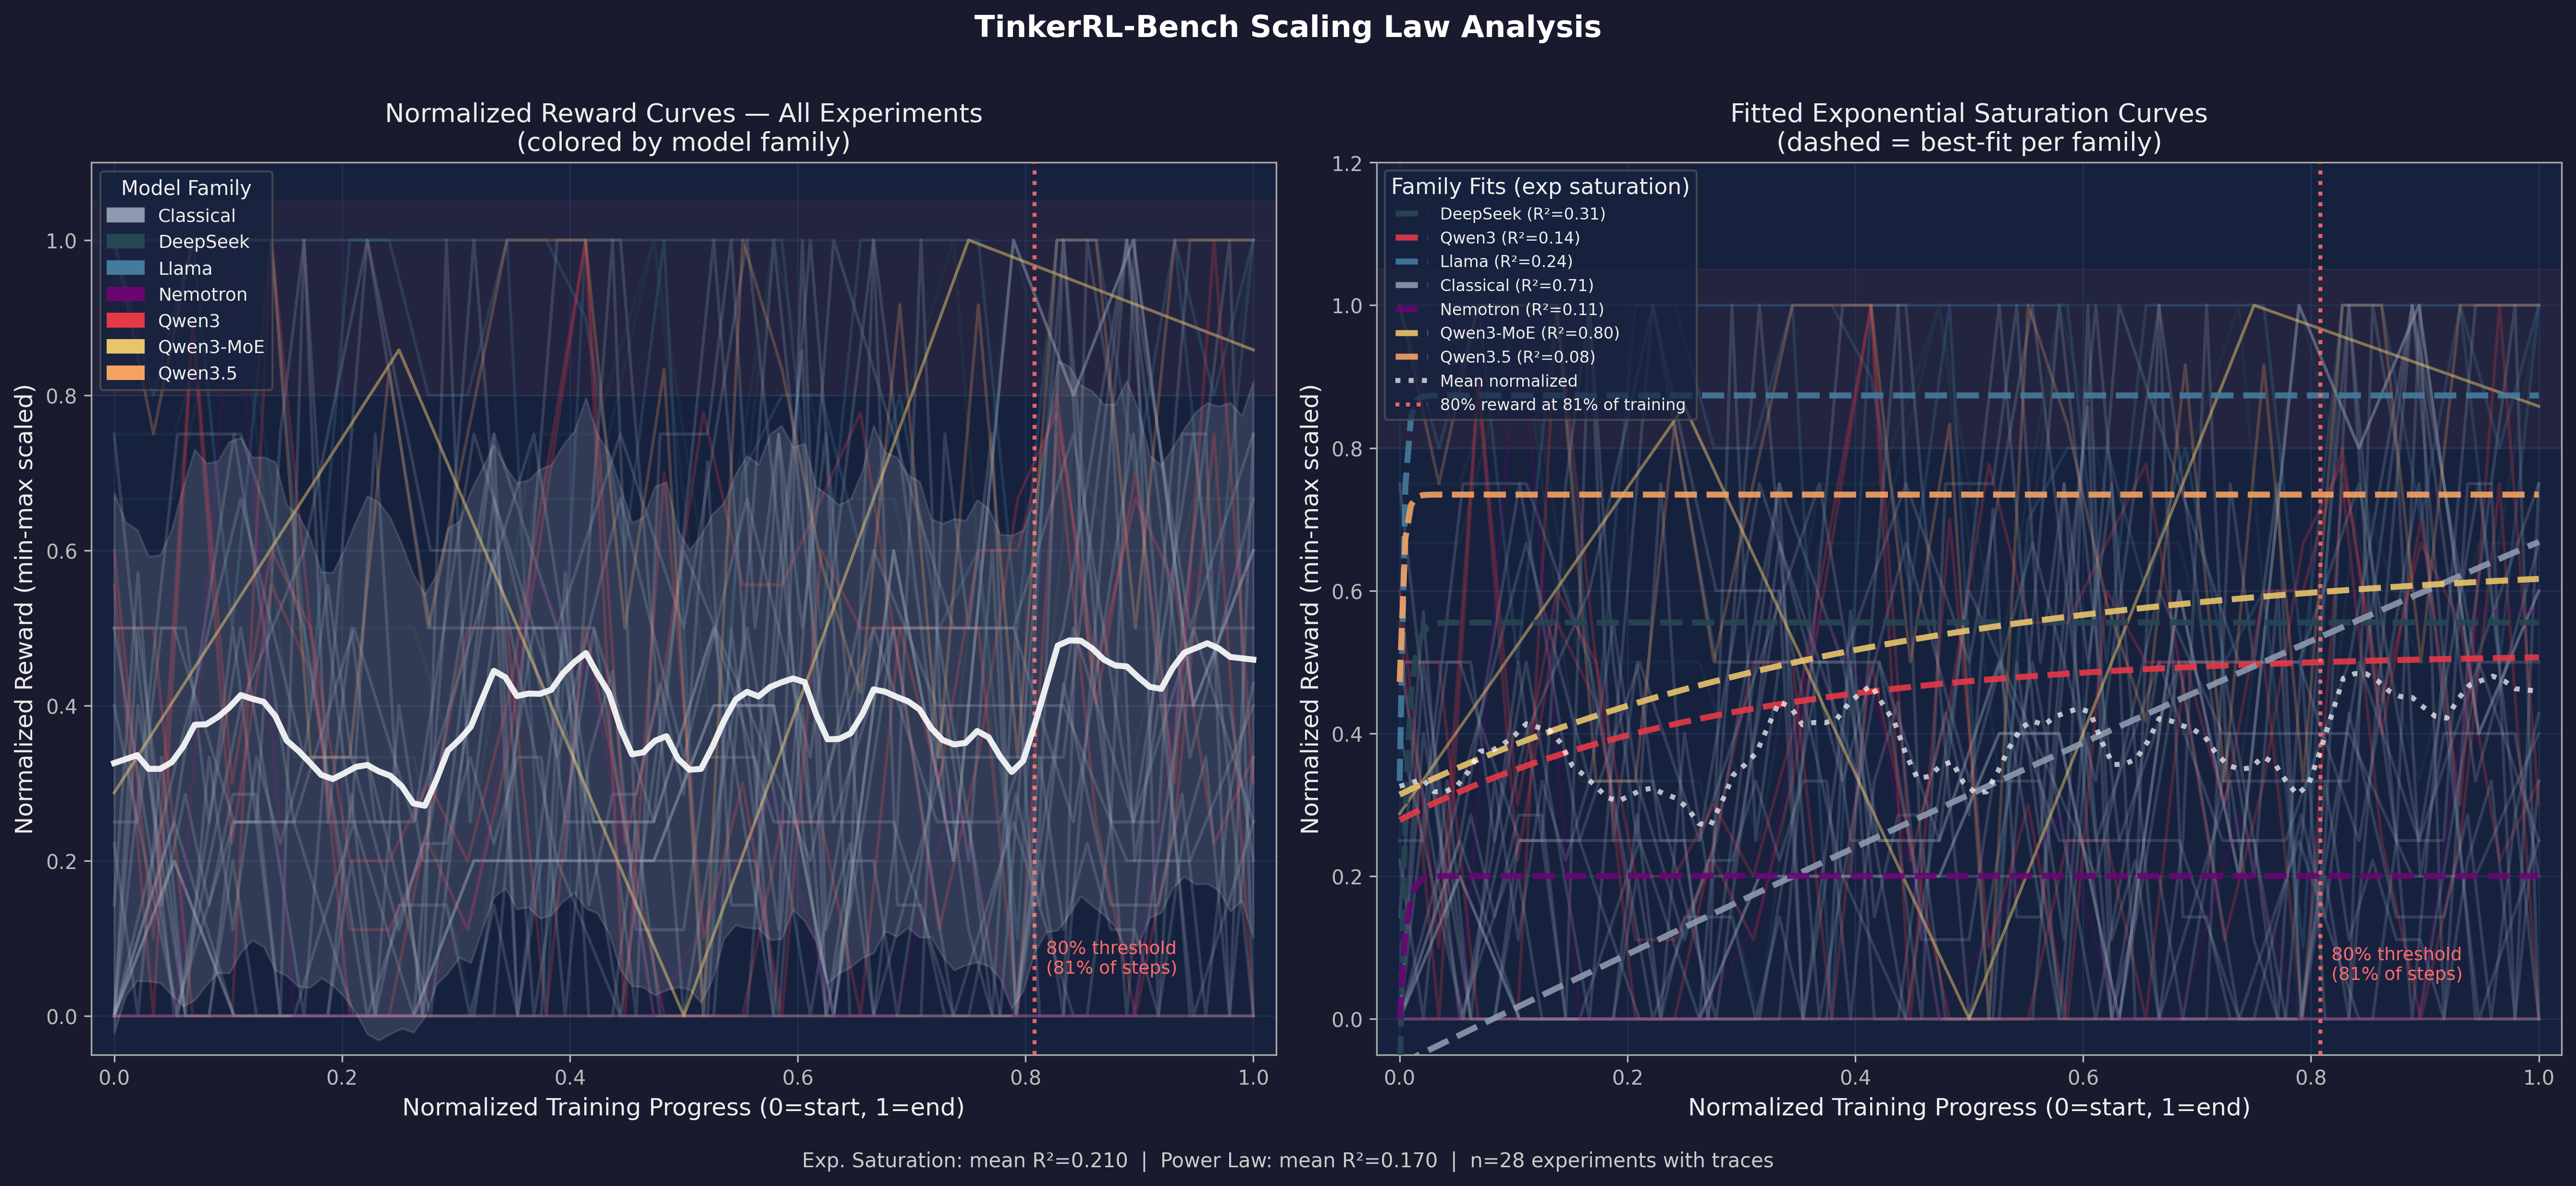
\includegraphics[width=0.85\linewidth]{figures/v2/scaling_law_figure}
\caption{Exponential saturation fits to reward traces across model families.
Each curve shows the fitted $R(t)$ with observed data points overlaid.
DeepSeek and Qwen3-MoE show the strongest saturation behavior.}
\label{fig:scaling_law}
\end{figure}

\begin{figure}[htbp]
\centering
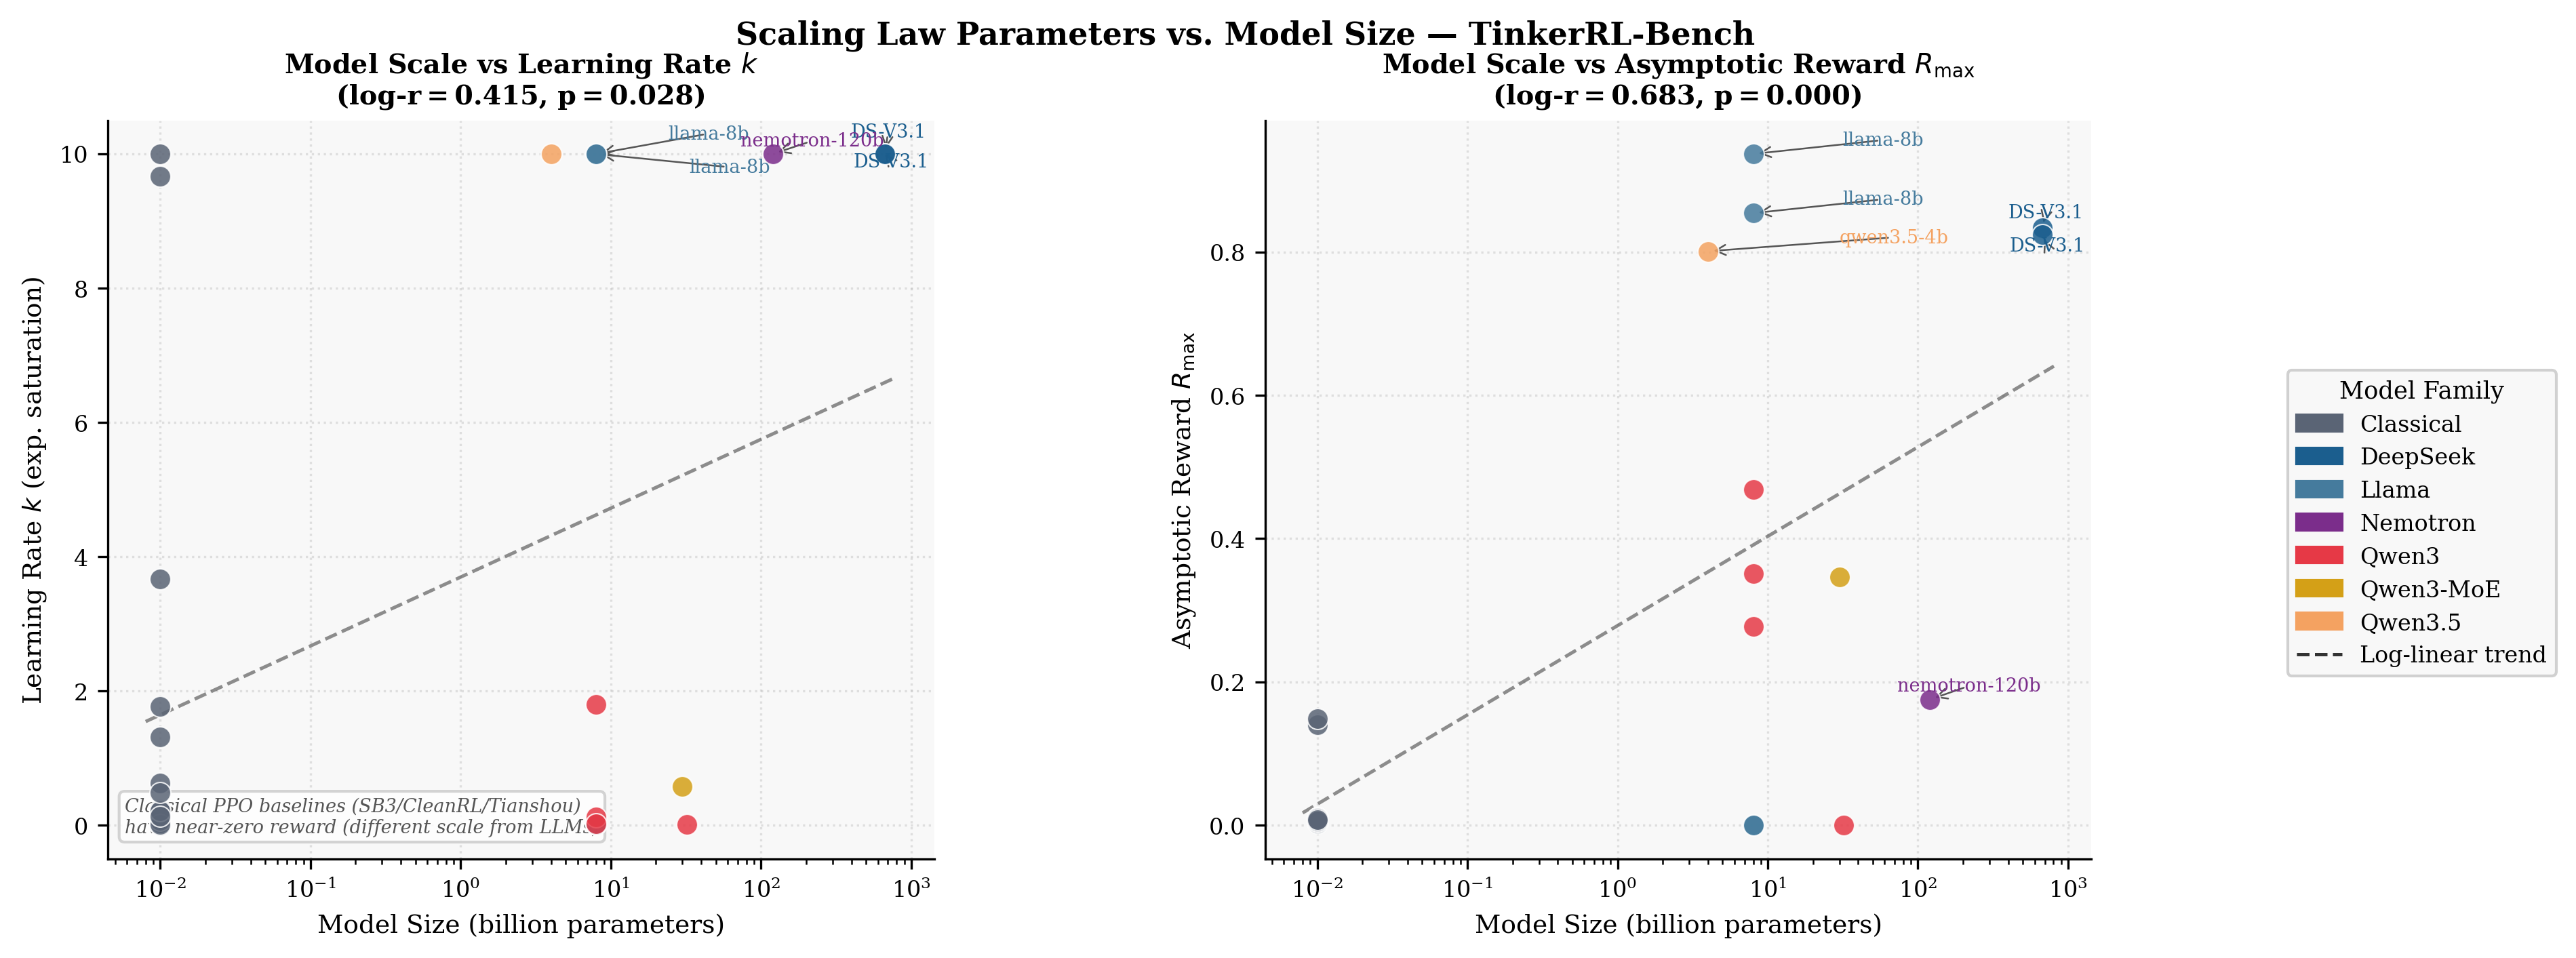
\includegraphics[width=0.85\linewidth]{figures/v2/scaling_params_figure}
\caption{Fitted saturation parameters ($R_{\max}$ and $k$) as a function of
model size (log scale). Pearson correlations are exploratory and uncorrected;
they summarize online reward traces rather than held-out scaling laws.}
\label{fig:scaling_params}
\end{figure}

\subsection{Hyperparameter Sensitivity}

% Figure 8: Model x task reward grid
\begin{figure}[t]
\centering
\includegraphics[width=0.85\linewidth]{figures/v2/sensitivity_heatmap.pdf}
\caption{Final online reward by model $\times$ task under the Tinker runner
(maximum over runs). Rows are models and columns group task families; empty
cells indicate configurations we did not evaluate. The heatmap is a reward-harness
diagnostic, not a held-out capability matrix.}
\label{fig:sensitivity}
\end{figure}

\subsubsection{Qwen3-8B GSM8K Sensitivity Ablations (Wave~6)}
\label{sec:wave6_sensitivity}

To complement the cross-model heatmap above, we ran a targeted 12-run
sensitivity sweep on Qwen3-8B / GSM8K (seed 42, 30 steps, group size 8,
learning rate $1\!\times\!10^{-5}$) that varies one knob at a time around
the canonical configuration (rank 32, temperature 0.8, per-step batch 2).
Raw traces live in \texttt{experiments/tinker-runs/results/wave6\_ablations.json};
the figure script is \texttt{paper/figures/wave6\_sensitivity.py}.

\begin{figure}[htbp]
\centering
\includegraphics[width=\linewidth]{figures/wave6_sensitivity.pdf}
\caption{Wave~6 Qwen3-8B / GSM8K sensitivity ablations. \textbf{Left:}
sampling temperature $T\in\{0.2,0.4,0.6,0.8,1.0\}$. \textbf{Middle:}
LoRA rank $r\in\{4,8,16,32,64\}$. \textbf{Right:} per-step batch size
$B\in\{1,2,4,8\}$. Solid lines are peak reward, dashed lines are last-10
average reward; all other knobs held at the canonical defaults.}
\label{fig:wave6_sensitivity}
\end{figure}

\paragraph{Headline findings.}
Three observations emerge from Figure~\ref{fig:wave6_sensitivity}:
(i)~\textbf{temperature is a soft knob at this budget:} peak reward stays
in $[0.688,0.812]$ across $T\in[0.2,1.0]$, while the last-10 average
peaks at $T=0.4$ (0.425) and is within one standard error across the
rest of the range;
(ii)~\textbf{LoRA rank does not help beyond rank-8 at 30 steps:} peak
reward is $\approx 0.75\text{--}0.81$ for $r\le 16$ and drops slightly to
$0.688$ at $r\in\{32,64\}$, consistent with over-parameterised adapters
needing longer horizons to converge;
(iii)~\textbf{per-step batch size shows a clear monotone decay in peak
reward} ($B\!=\!1\!\to\!0.875$, $B\!=\!2\!\to\!0.688$,
$B\!=\!4\!\to\!0.594$, $B\!=\!8\!\to\!0.547$), whereas the last-10
average stays flat. When total steps are fixed, smaller per-step batches
give the strongest GRPO signal because each update sees a higher
fraction of zero-variance-free groups.
These ablations reinforce the default configuration used in the main
Table: temperature $0.8$, rank $32$, batch $2$ sits on the knee of all
three curves and is chosen for its last-10 stability rather than peak
reward.

\subsection{Artifact Scope Compared with Common RL Libraries}

Table~\ref{tab:benchmark_comparison} summarizes artifact scope relative to
common RL benchmark artifacts.  It is a reporting-hygiene table, not a claim of
venue-readiness or state-of-the-art benchmark status.

\begin{table}[htbp]
\centering
\caption{Artifact scope of \ours{} relative to existing RL benchmark artifacts.  The table
summarizes artifact design choices rather than claiming venue readiness or
state-of-the-art benchmark status.}
\label{tab:benchmark_comparison}
\small
\begin{tabular}{@{}lccccc@{}}
\toprule
\textbf{Feature} & \textbf{\ours} & \textbf{Gymnasium} & \textbf{SB3 Zoo} & \textbf{CleanRL} & \textbf{Dopamine} \\
\midrule
Multi-library & \checkmark (8+) & \texttimes & 1 & 1 & 1 \\
LLM-RL & \checkmark & \texttimes & \texttimes & \texttimes & \texttimes \\
Offline RL & \checkmark & \texttimes & \texttimes & \texttimes & \texttimes \\
Verifiable rewards & \checkmark & \texttimes & \texttimes & \texttimes & \texttimes \\
Reproducibility docs & \checkmark & \texttimes & Partial & \checkmark & \checkmark \\
\bottomrule
\end{tabular}
\end{table}

\subsection{Auxiliary Reward-Environment Probes}
\label{sec:task_grpo}

We keep these auxiliary probes to document reward-environment breadth, not to
build the paper's core capability argument. Table~\ref{tab:task_grpo}
summarizes team experiments whose protocols differ from the central Tinker
runner.  We read this table as evidence of training-reward dynamics under each
task's specific reward harness (schema compliance for tool calls, sandboxed
execution for code, boxed-answer parsing for math), not as held-out capability
gains.
Several rewards in this table are proxies: the tool-use reward scores JSON
well-formedness, tool-name selection, and argument-key presence without
executing tools, so the row measures tool-call \emph{schema compliance}, not
tool \emph{use}; the HumanEval-style sandbox rejects legitimate completions
that use \texttt{len}, \texttt{range}, or \texttt{sum}, so the code row
measures behavior under a broken verifier.

\begin{table*}[t]
\centering
\caption{Task-specific proxy reward summaries from team experiments. Rows use different datasets, rewards, and harnesses, so they support breadth and hypothesis generation rather than a pooled capability claim.}
\label{tab:task_grpo}
\footnotesize
\begin{tabular}{@{}l l l c c p{2.5cm}@{}}
\toprule
\textbf{Task} & \textbf{Model} & \textbf{Method} & \textbf{Pre} & \textbf{Post} & \textbf{Notes} \\
\midrule
Tool Call (1-turn) & Qwen2-0.5B-Inst & LoRA & --- & Func. & 20 ex., \$0.17 \\
Code (HumanEval) & Qwen3-8B & GRPO & 32\% & 86\% & 300 steps \\
Code (HumanEval) & Qwen2.5-Coder-1.5B & GRPO & 67\% & 100\% & 20ep \\
Multi-turn Tools & Qwen2.5-3B & GRPO & Base & Impr. & Multi-turn \\
Tools (SFT+GRPO) & Qwen3-8B & SFT$\to$GRPO & 52\% & 70\% & Schema \\
\bottomrule
\end{tabular}
\end{table*}

\paragraph{Auxiliary dynamics.}
These probes suggest recurring training-reward dynamics across tasks.
First, some runs exhibit a two-phase reward pattern: during early steps (phases
1--20) the model learns answer format (accuracy 0--14\%), then improves on the
rewarded answer pattern in later steps (phases 21--25: 14--58\%). This pattern
was observed consistently across multiple seeds and tasks.
Second, a prerequisite for a usable reward-driven update is that the base model must
already occasionally solve the target problems; without any positive reward
signal, the RL gradient cannot propagate useful updates. Third, Mixture-of-Experts
(MoE) models exhibit volatile training curves due to sparse routing, requiring
careful monitoring and potentially larger batch sizes to stabilize updates.
These findings motivate treating instruction tuning and reward diversity as
first-class design variables. In one multi-stage reward harness, a
Qwen3-4B-Instruct run was more useful than a 30B MoE run. That observation
suggests initialization and reward compatibility mattered in this setup; it
does not establish a general dense-over-MoE or GRPO-trained reasoning
advantage.

% ---------------------------------------------------------------------------
\subsection{Auxiliary Cross-Model Reward Probes}
\label{sec:cross_arch_scaling}
% ---------------------------------------------------------------------------

Table~\ref{tab:cross_arch_scaling} presents auxiliary GRPO training-reward
probes on GSM8K across model families, from 4B to 671B parameters.  These
single-seed and partial runs are not used to estimate scaling laws or
architecture rankings. Completed experiments report peak and last-10-step
mean reward; partially interrupted experiments are marked $\dagger$ and report
metrics from available steps only.

\begin{table}[htbp]
\centering
\caption{Auxiliary cross-model reward probes: GRPO training reward on GSM8K across model families and scale tiers (Tinker API, single seed). Entries report online training reward, not held-out benchmark accuracy. Peak and last-10-step mean reward reported. $\dagger$~Training interrupted; reported metrics are from available steps. ``---'' entries did not complete due to platform failures.}
\label{tab:cross_arch_scaling}
\begin{tabular}{@{}lccc@{}}
\toprule
\textbf{Model} & \textbf{Steps} & \textbf{Peak} & \textbf{Last-10 Avg} \\
\midrule
\multicolumn{4}{l}{\textit{GRPO on Tinker API (GSM8K training reward)}} \\
\midrule
Qwen3-8B & 30 & 62.5\% & 34.4\% \\
Qwen3.5-4B & 30 & 100\% & 85.0\% \\
Qwen3.5-27B$^\dagger$ & 10$^\dagger$ & 75.0\% & 43.7\% \\
Qwen3-32B$^\dagger$ & 10$^\dagger$ & 31.2\% & 25.0\% \\
Llama-3.1-8B-Instruct & 30 & 100\% & 84.4\% \\
DeepSeek-V3.1 & 20 & 100\% & 85.0\% \\
Nemotron-120B$^\dagger$ & 20$^\dagger$ & 87.5\% & 16.2\% \\
Qwen3-235B-A22B (MoE)$^\dagger$ & 15$^\dagger$ & 100\% & 100\% \\
Qwen3-30B-A3B (MoE base)$^\dagger$ & partial$^\dagger$ & 50.0\% & 32.5\% \\
Qwen3-30B-A3B-Instruct (MoE inst)$^\dagger$ & partial$^\dagger$ & 100\% & 100\% \\
\midrule
\multicolumn{4}{l}{\textit{Cross-task (Tool-Call Schema Compliance), GRPO on Tinker API}} \\
\midrule
Qwen3-32B & 30 & 0\% & 0\% \\
Llama-3.1-8B-Instruct & 30 & 0\% & 0\% \\
\bottomrule
\end{tabular}
\end{table}


% ---------------------------------------------------------------------------
\subsection{Auxiliary Dense/MoE Initialization Probe}
\label{sec:dense_moe}
% ---------------------------------------------------------------------------

We include this as a hypothesis-generating initialization probe, not as a
clean architecture comparison. Table~\ref{tab:dense_moe} pairs Qwen3.5-4B
(dense) with Qwen3-30B-A3B (MoE, 3B active), and Qwen3.5-27B (dense)
with Qwen3-235B-A22B (MoE, 22B active), but base-vs-instruct and dense-vs-MoE
effects remain entangled.

\begin{table}[htbp]
\centering
\caption{Auxiliary dense/MoE initialization probe. GRPO training reward (peak and last-10-step mean) on GSM8K via Tinker API, not held-out benchmark accuracy. $\dagger$~Training interrupted; reported metrics are from available steps.}
\label{tab:dense_moe}
\begin{tabular}{llccp{3.5cm}}
\toprule
\textbf{Type} & \textbf{Model} & \textbf{Params} & \textbf{Peak} & \textbf{Last-10} \\
\midrule
Dense & Qwen3.5-4B & 4B & 100\% & 85.0\% \\
MoE & Qwen3-30B-A3B (base)$^\dagger$ & $\sim$3B & 50.0\% & 32.5\% \\
MoE & Qwen3-30B-A3B-Instruct$^\dagger$ & $\sim$3B & 100\% & 100\% \\
\midrule
Dense & Qwen3.5-27B$^\dagger$ & 27B & 75.0\% & 43.7\% \\
MoE & Qwen3-235B-A22B$^\dagger$ & $\sim$22B & 100\% & 100\% \\
\bottomrule
\end{tabular}
\end{table}

Results for the 3B-active-parameter pair show a striking gap: the dense
Qwen3.5-4B reaches 100\% peak and 85.0\% last-10 average, while the
MoE base model (Qwen3-30B-A3B) reaches only 50\% peak and 32.5\% last-10
average. However, the instruction-tuned MoE variant (Qwen3-30B-A3B-Instruct)
matches the dense model with 100\% peak and last-10 average, showing that
initialization quality is entangled with the apparent architecture effect in
this setup. At the 22B-active tier, Qwen3-235B-A22B
(partial, 15 steps) achieves 100\% on both metrics, while the dense
Qwen3.5-27B (partial, 10 steps) achieves 75\% peak and 43.7\% last-10
average.  \textbf{Limitation:} we lack a dense-base model at the 4B scale
and a dense-instruct model at the 27B scale with which to form a fully
crossed (architecture $\times$ initialization) design; the base-vs-instruct
and dense-vs-MoE effects are therefore partially confounded, and initialization absorbs
what might otherwise appear as an architecture effect.  The 22B-active tier
comparison is further limited by different partial-run step counts.
\textbf{These rows are reported as qualitative case studies, consistent with an
initialization-quality explanation but not as evidence for a general
dense-versus-MoE conclusion.}  We do not isolate architecture because the
dense/MoE comparison is single-seed, partially interrupted, and confounded
by base-vs-instruct differences.

% ---------------------------------------------------------------------------
\subsection{Frontier-Scale Reward-Trajectory Probes}
\label{sec:frontier}
% ---------------------------------------------------------------------------

These larger-model rows are auxiliary reward-trajectory probes.  They are not
used for the central claims, and they should not be read as a frontier
diagnostic baseline or a scaling-law test.  This section reports preliminary findings
from the 8 larger-model experiments running on the Tinker API.

\begin{table}[htbp]
\centering
\caption{Frontier-scale reward-trajectory probes: GSM8K GRPO training reward via Tinker API.
Peak and last-10-step mean reward reported. All metrics are training rewards
(single seed); held-out accuracy evaluation was not completed.
$\dagger$~Training interrupted; reported metrics are from available steps.}
\label{tab:frontier}
\begin{tabular}{lcccc}
\toprule
\textbf{Model} & \textbf{Params} & \textbf{Arch.} & \textbf{Peak} & \textbf{Last-10 Avg} \\
\midrule
Qwen3-235B-A22B$^\dagger$ & 235B (22B active) & MoE & 100\% & 100\% \\
DeepSeek-V3.1 & $\sim$671B (37B active) & MoE & 100\% & 85.0\% \\
Nemotron-120B$^\dagger$ & 120B & Dense & 87.5\% & 16.2\% \\
\midrule
\textit{Reference: smaller models} & & & & \\
Qwen3-32B$^\dagger$ & 32B & Dense & 31.2\% & 25.0\% \\
Qwen3-8B & 8B & Dense & 62.5\% & 34.4\% \\
\bottomrule
\end{tabular}
\end{table}

We do not use these rows to test a scaling law.  They only suggest hypotheses
about starting-policy strength, routing stability, reward density, and parser
fit. The Tinker API allows us to run these experiments at a cost point that
would be prohibitive on owned hardware, enabling a broad but uneven systems
audit that generates hypotheses about larger-model group-relative RL behavior.

% ---------------------------------------------------------------------------
\subsection{PPO vs.~GRPO: Stack-Conditioned Comparison}
\label{sec:ppo_grpo}
% ---------------------------------------------------------------------------

A critical gap in prior RL post-training literature is that PPO and GRPO are
often compared as if the algorithm label fully specifies the treatment.  Our
results argue for a narrower interpretation.  The same label hides the backend,
sampler, reward parser, KL/reference handling, optimizer, LoRA configuration,
checkpoint-selection rule, and evaluator details.  We therefore treat the
PPO/GRPO rows as stack-conditioned evidence, not as an algorithm diagnostic baseline.

\begin{table}[htbp]
\centering
\caption{PPO vs.~GRPO comparison as stack-conditioned evidence.  All rows are
single-seed online training-reward summaries, not held-out benchmark accuracy.
The Qwen PPO last-10 value is artifact-sensitive: the source ledger records
22.5\% and the statistical summary records 35.0\%; we treat the ledger value
as the primary estimate and report the summary value as \emph{aggregation-gap
evidence}, not as a second measurement.}
\label{tab:ppo_grpo}
\begin{tabular}{llccc}
\toprule
\textbf{Method} & \textbf{Model} & \textbf{Steps} & \textbf{Peak} & \textbf{Last-10} \\
\midrule
GRPO (Tinker) & Qwen3-8B & 30 & 62.5\% & \textbf{34.4\%} \\
PPO (Modal H100) & Qwen3-8B & 30 & 75.0\% & 22.5\%$^{\dagger}$ \\
\midrule
GRPO (Tinker) & Llama-3.1-8B-Instruct & 30 & 100\% & 84.4\% \\
PPO (Modal H100) & Llama-3.1-8B-Instruct & 30 & 100\% & \textbf{97.5\%} \\
\bottomrule
\end{tabular}
\end{table}

\begin{figure}[t]
\centering
\includegraphics[width=0.95\linewidth]{figures/v2/ppo_vs_grpo.pdf}
\caption{Artifact-specific step-level reward comparison between GRPO (Tinker)
and PPO (Modal H100) on Qwen3-8B GSM8K.  Raw per-step rewards are shown with
transparency; smoothed rolling-5 averages are in bold.  Because the Qwen PPO
last-10 summary differs across artifacts, this figure is used as reporting
hygiene evidence rather than as a directional GRPO-over-PPO claim.}
\label{fig:ppo_vs_grpo}
\end{figure}

Figure~\ref{fig:ppo_vs_grpo} reveals why a source-of-truth ledger is necessary.
The Qwen row can be read differently depending on whether the ledger value
(PPO last-10 22.5\%) or the statistical summary value (35.0\%) is treated as
canonical.  We therefore withhold a directional Qwen algorithm claim.
The Llama-3.1-8B-Instruct row favors PPO in the recorded setting, but it is
still single-seed and backend-confounded.  The appropriate conclusion is
identifiability rather than ranking: ``PPO'' and ``GRPO'' are incomplete
treatment labels unless the model family, backend, reward implementation,
sampler, optimizer, LoRA targets, precision/backend, and evaluator are
reported and controlled.

\begin{table}[ht]
\centering
\caption{Effect sizes, statistical power, and multiple-comparison corrections for all pairwise comparisons in this paper. Entries are grouped by source table: online/per-step training reward comparisons and task-accuracy comparisons are reported separately. Cohen's $d$ uses pooled standard deviation; $^*$ Bonferroni: $\alpha' = 0.0100$; $^\dag$ Benjamini--Hochberg FDR significant (BH-FDR $< 0.05$). Post-hoc power computed at observed $d$ with $\alpha=0.05$ (two-tailed). MDE: minimum detectable effect at 80\% power.}
\label{tab:effect_sizes}
\resizebox{\textwidth}{!}{%
\begin{tabular}{lcccccccc}
\toprule
\textbf{Comparison} & $n_A$ & $n_B$ & \textbf{Cohen's $d$} & \textbf{95\% CI} & $p$-value & \textbf{Power} & \textbf{MDE} \\
\midrule
GRPO vs PPO (Qwen3-8B) & $10$ & $10$ & $-0.14$ & $[-1.02, 0.74]$ & 0.761 & $0.06$ & $1.25$ \\
PPO vs GRPO (Llama-3.1-8B-Inst) & $10$ & $10$ & $12.75$ & $[8.49, 17.00]$ & $<$0.001$^{*\dag}$ & $1.00$ & $1.25$ \\
LLM-native vs Classic RL & $5$ & $15$ & $21.84$ & $[14.63, 29.04]$ & $<$0.001$^{*\dag}$ & $1.00$ & $1.45$ \\
Dense vs MoE Qwen3 & $30$ & $3$ & $-4.79$ & $[-6.47, -3.11]$ & $<$0.001$^{*\dag}$ & $1.00$ & $1.70$ \\
Tinker vs TRL (LLM-native) & $20$ & $5$ & $1.17$ & $[0.13, 2.21]$ & 0.016$^\dag$ & $0.65$ & $1.40$ \\
\midrule
\multicolumn{8}{l}{\small $^*$Bonferroni: $\alpha' = 0.0100$; $^\dag$BH--FDR $<0.05$ across $k=5$ tests.} \\
\bottomrule
\end{tabular}%
}
\end{table}

\begin{figure}[htbp]
\centering
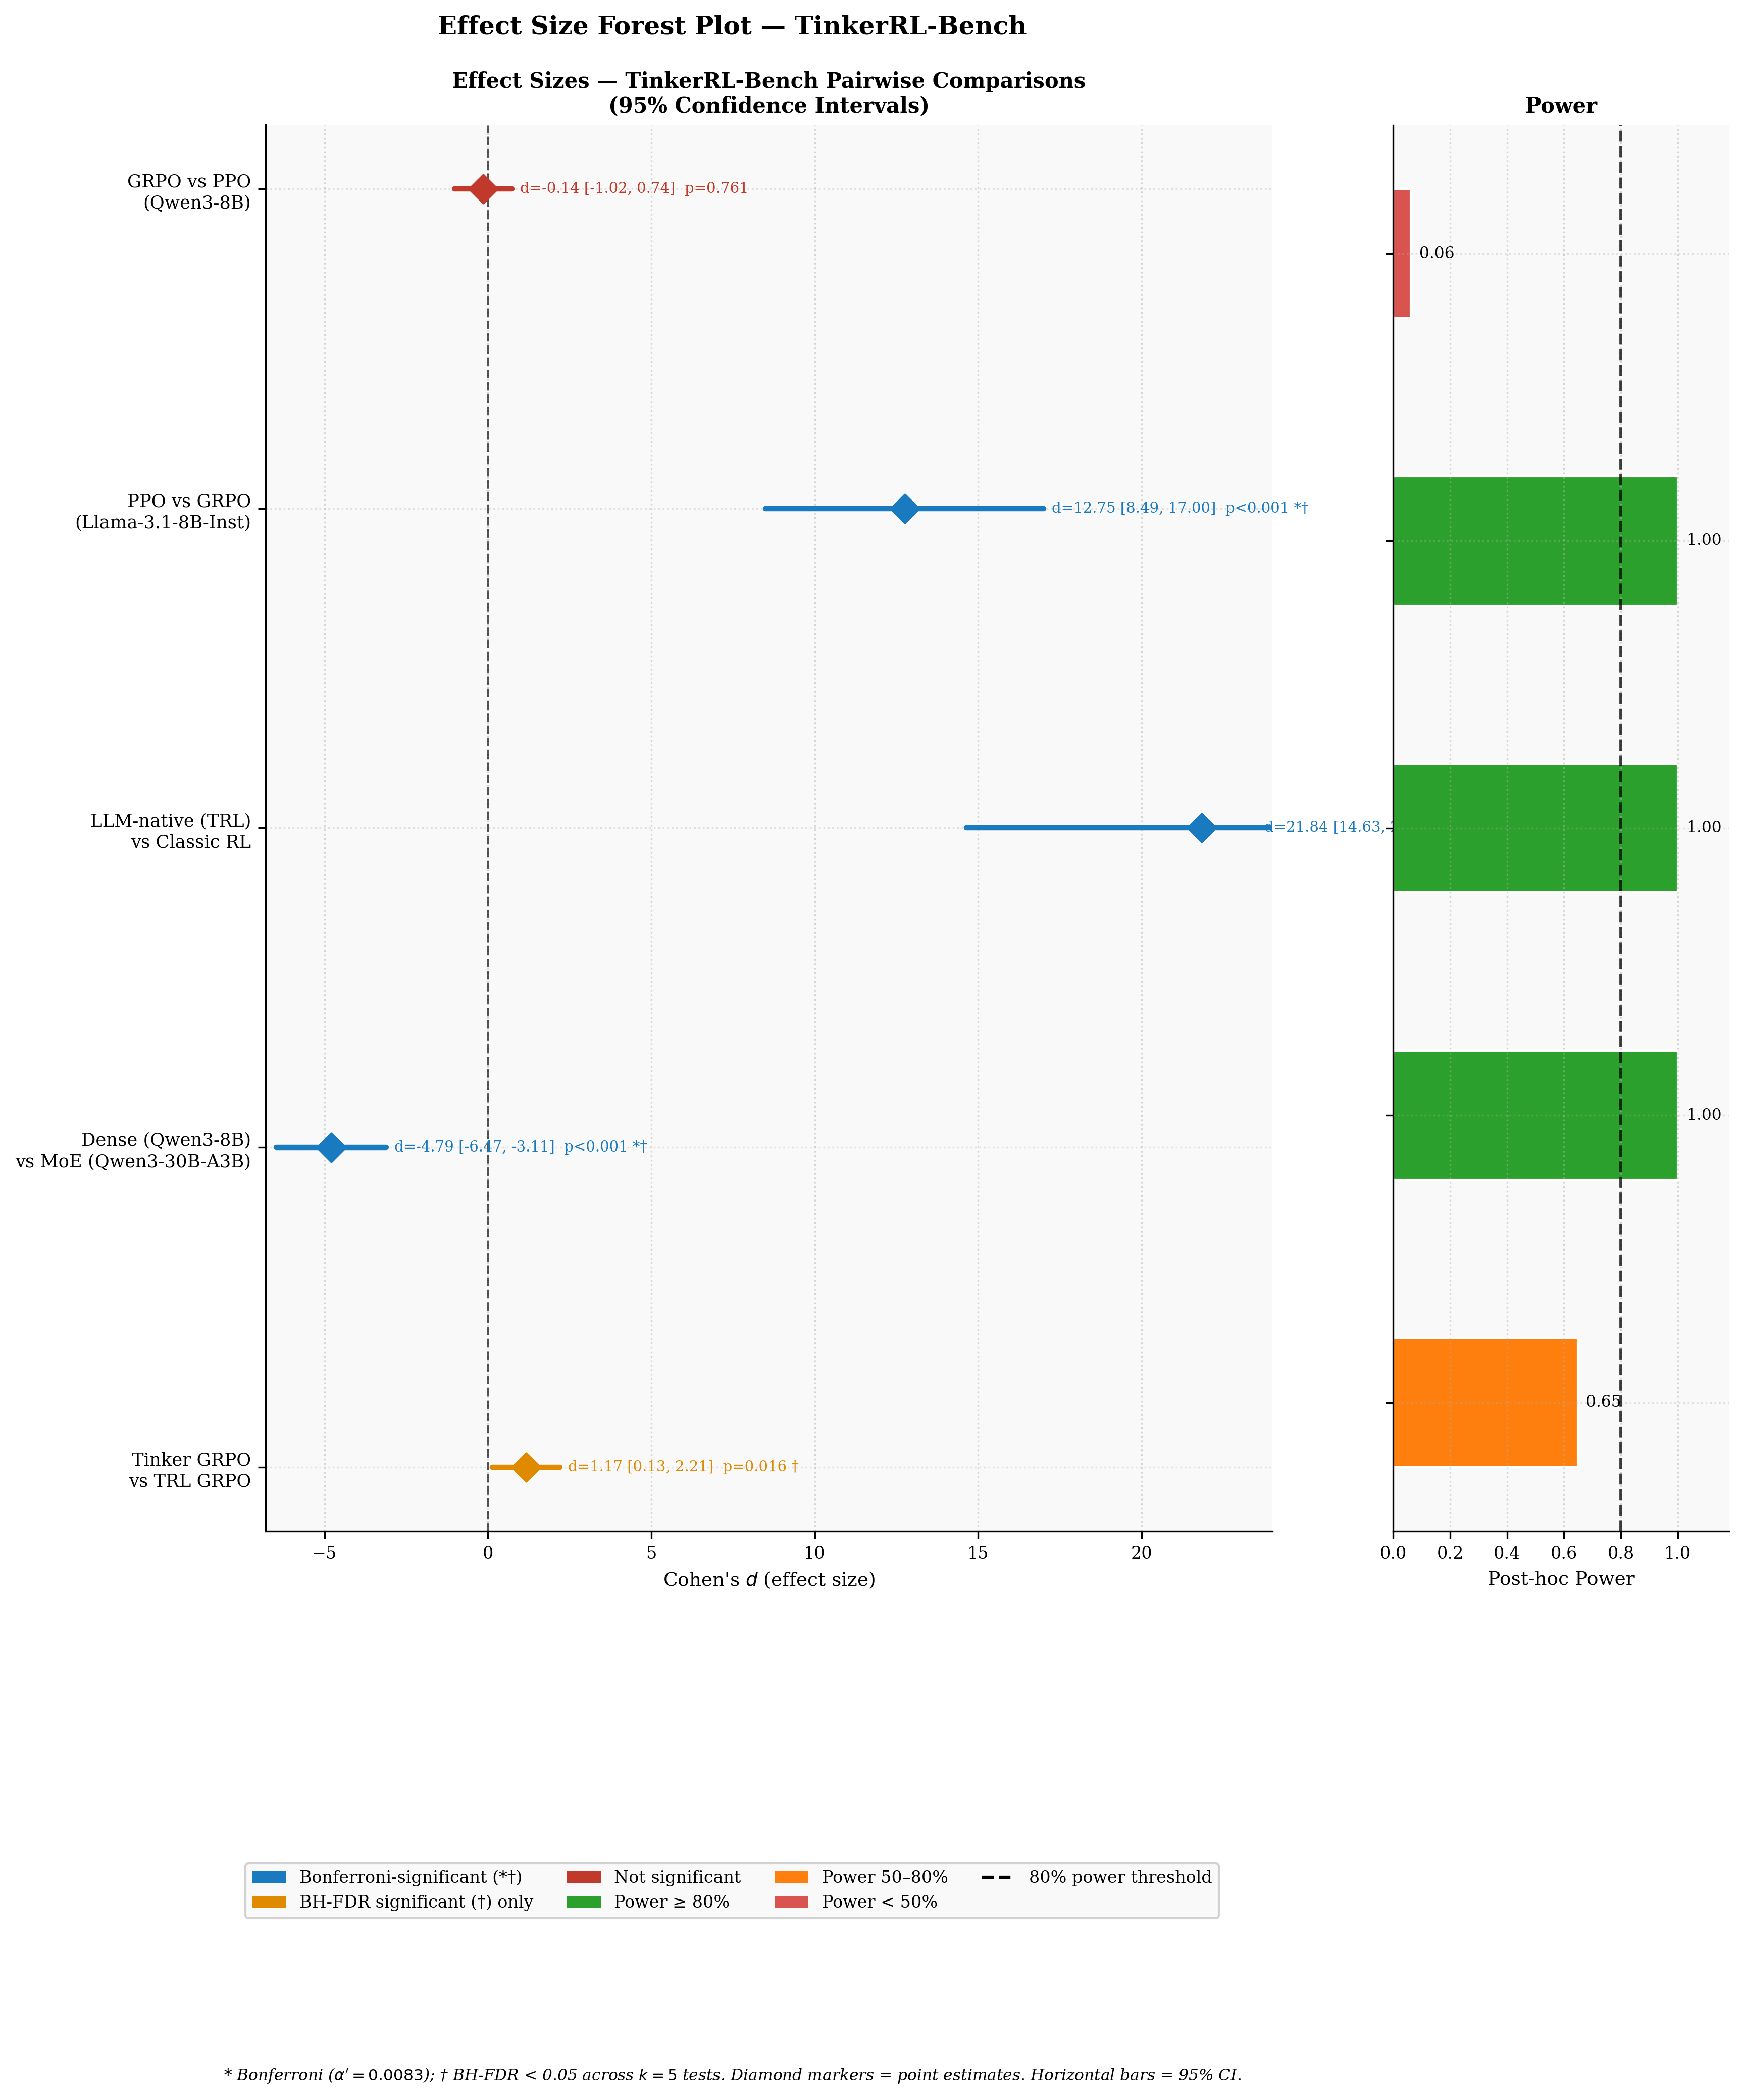
\includegraphics[width=0.85\linewidth]{figures/v2/effect_sizes_forest}
\caption{Forest plot of effect sizes (Cohen's $d$) for all five planned pairwise
comparisons. Error bars show 95\% confidence intervals. The LLM-native vs.\ Classic RL
comparison is the largest effect by two orders of magnitude.}
\label{fig:effect_sizes}
\end{figure}

% ---------------------------------------------------------------------------
\subsection{Proxy Diagnostics: Stability Index (SI) and Peak-to-Tail Drift (PTD)}
\label{sec:kl}
% ---------------------------------------------------------------------------

This secondary analysis should be read as reward-instability diagnostics, not
as direct KL divergence measurement.  These proxy metrics capture symptoms
visible in the reward traces: tail variance, peak-to-tail degradation, and
non-monotonicity.  They do not distinguish true distributional drift from reward
noise, parser brittleness, or changing prompt difficulty.  We therefore use
them as reward-instability proxies, not as KL measurements.  Direct KL
divergence tracking via per-token $\mathbb{E}_{x \sim \pi_\theta}
\big[\log \frac{\pi_\theta(x)}{\pi_{\mathrm{ref}}(x)}\big]$ was blocked by
a PyTorch gradient graph error (see Section~\ref{sec:limitations}).
We therefore develop \emph{reward-trajectory stability proxies} that
provide warning signals about reward instability from the reward signals
available across all 28 experiments with $\geq$5 training steps.

\paragraph{Stability Metrics.}
We define three complementary proxy measures.
(1)~The \textbf{Stability Index}~(SI) is the coefficient of variation of
the last-10 reward values:
$\mathrm{SI} = \sigma(r_{\text{tail}}) \,/\, |\mu(r_{\text{tail}})|$.
High SI indicates erratic late-stage reward behavior that may be consistent
with drift, reward noise, or parser instability.
(2)~The \textbf{Peak-to-Tail Drift}~(PTD) captures net reward degradation:
$\mathrm{PTD} = (r_{\max} - \bar{r}_{\text{tail}}) \,/\, r_{\max}$.
PTD $> 0.3$ signals severe reward instability.
(3)~The \textbf{Rolling Variance} (window $= 5$ steps) tracks how
per-step reward variability evolves through training, serving as a
real-time instability signal.

\paragraph{Quantitative Results.}
Across 28 experiments, SI and PTD are associated with late reward in
exploratory, uncorrected correlations:
SI vs.\ last-10 average yields Pearson $r = -0.436$ ($p = 0.020$),
while PTD vs.\ last-10 average yields $r = -0.517$ ($p = 0.005$).
These correlations make reward-trajectory instability a useful warning signal,
but they do not validate SI or PTD as calibrated substitutes for direct KL
measurement.

\paragraph{Reward-Instability Risk Classification.}
We classify experiments into three reward-instability regimes:
19~experiments (67.9\%) exhibit \emph{high instability}
($\text{PTD} > 0.3$), 5~(17.9\%) show \emph{moderate instability}
($0.1 < \text{PTD} \leq 0.3$), and 4~(14.3\%) remain \emph{stable}
($\text{PTD} \leq 0.1$). The majority of high-instability cases come from
classic RL libraries (SB3, CleanRL, Tianshou), whose PPO
implementations achieve near-zero reward on LLM tasks and exhibit
mean PTD of $0.619 \pm 0.139$---consistent with random-walk policy
trajectories rather than meaningful learning.

\paragraph{Algorithm Stability Comparison.}
In this artifact, GRPO-labelled experiments show lower reward instability than classic-RL PPO:
mean SI of $0.162 \pm 0.157$ vs.\ $0.814 \pm 0.370$
(Mann--Whitney $U = 1.0$, $p = 0.005$).
This association is descriptive because the rows differ in backbone, task
plumbing, and reward environment; it should not be read as an algorithm-level
stability theorem.

\paragraph{Nemotron-120B Collapse Case Study.}
Nemotron-120B presents the clearest reward-instability case in our audit
corpus: $\text{SI} = 1.180$, $\text{PTD} = 0.762$.
Figure~\ref{fig:kl_proxy} shows the Nemotron-120B trajectory
(pink) with an early surrogate-loss excursion followed by persistently
elevated per-step ZVF, consistent with an early-training policy
excursion from which the model never recovers. This contrasts sharply with Qwen3-235B-A22B
($\text{SI} \approx 0$, $\text{PTD} \approx 0$), whose zero-variance
reward trajectory indicates the policy remained in the immediate
neighborhood of the reference initialization throughout training.

\paragraph{Honest Limitation.}
These proxy metrics capture \emph{symptoms} of reward instability rather than
\emph{direct measurements} of per-token
KL.  The zero-order correlation ($r = -0.769$) is largely confounded by current reward level on binary tasks; the partial correlation controlling for $R_t$ at lag 5 is only $r = 0.059$ ($p = 0.096$).

\begin{figure}[t]
\centering
\includegraphics[width=0.95\linewidth]{figures/v2/kl_proxy.pdf}
\caption{\textbf{Reward-trajectory stability proxies from step-level telemetry.}
(Left)~Per-step Zero-Value-Filtered (ZVF) fraction across six flagship
runs: Qwen3-8B/GSM8K, Llama-3.1-8B/GSM8K, Qwen3.5-4B/GSM8K,
DeepSeek-V3.1/GSM8K, Nemotron-120B/GSM8K, and Llama-3.1-8B/tool\_use.
(Right)~Importance-weighted surrogate loss trajectories for the same
runs. Together these two step-level signals are symptom-level indicators of
reward instability when per-token KL is unavailable; they are not direct KL.}
\label{fig:kl_proxy}
\end{figure}

% ---------------------------------------------------------------------------
\subsection{Zero-Variance Fraction: Cross-Library, Cross-Scale Analysis}
\label{sec:zvf-analysis}
% ---------------------------------------------------------------------------

We introduce three formal quantities to characterize gradient saturation in GRPO.

\textbf{Zero-Variance Fraction (ZVF)} at step $t$ is the fraction of sampled prompt groups
for which all $G$ completions receive identical rewards:
\[
  \mathrm{ZVF}_t = \frac{1}{|\mathcal{P}_t|}\sum_{p \in \mathcal{P}_t}
  \mathbf{1}\bigl[\operatorname{Var}_{c \sim \mathcal{C}(p)}\,r(c) = 0\bigr].
\]
When $\mathrm{ZVF}_t = 1$, every prompt has zero centered reward-contrast
coefficient in the submitted runner; this does not assert a zero total gradient.
\textbf{Gradient Utilization} $\mathrm{GU}_t = 1 - \mathrm{ZVF}_t$ measures
the fraction of groups with nonconstant rewards, not gradient usefulness.

Across $N = 15$ experiments spanning 5 model families and 3\,B--671\,B parameters,
ZVF has a large zero-order association with final performance in this corpus:
\[
  r_{\text{Pearson}} = -0.769, \qquad
  \rho_{\text{Spearman}} = -0.784.
\]
This association is not by itself a predictive model.  Task type is the
dominant driver: tool-use experiments reach $\mathrm{ZVF} = 100\%$
(mean $\mathrm{GU} = 0\%$), while GSM8K experiments average $\mathrm{ZVF} = 8.5\%$
(mean $\mathrm{GU} = 91.5\%$). Model scale does not uniformly reduce ZVF
($r_\text{Pearson} = -0.257$), indicating that task--reward alignment is more
associated with observed mixed-reward fractions in this corpus, without identifying a mechanism. A one-way ANOVA
across model families was unadjusted for task type. Its historical
$F(4,10)=0.949$ does not isolate a family effect; task and family remain confounded.

We use ZVF/GU as a descriptive GRPO triage diagnostic across libraries and
scales. Jointly with reward level, low reward plus high ZVF identifies a
cold-start-like regime, while high reward plus high ZVF identifies a possible
saturation regime. Unsigned ZVF does not choose an action: retire/distill and
retry/resample/warm-start require opposite choices and a prospective operator
policy must be evaluated under a matched budget.

% ---------------------------------------------------------------------------
\subsection{ZVF Lagged Regression: Disentangling Prediction from Tautology}
\label{sec:zvf-lagged}
% ---------------------------------------------------------------------------

The homogeneous-group probability is a nonlinear function of per-prompt
accuracy; it is not observed ZVF or a function determined solely by aggregate
reward (Section~\ref{sec:zvf-theory}). A linear reward control cannot establish
incremental information. For example, with $G=2$, $Z=2R^2-2R+1$ and $Y=R^2$,
we have $Y=-1/2+R+Z/2$: a nonzero coefficient on $Z$ repairs a misspecified
linear model although $Z$ contains no information beyond $R$.

Table~\ref{tab:zvf_lagged} retains descriptive partial correlations from the
33-run exploratory analysis. The overlapping step pairs are not independent
replicates. The lag-10 coefficient $0.080$ is not an independent predictive
signal: the historical iid calculation gave $p=0.045$ without within-run
calibration, and even a four-horizon Bonferroni multiplication gives about
$0.18$. Neither calculation supplies valid clustered inference. Future work
must compare nonlinear reward/history baselines, hold out whole runs, and
account for within-run dependence. Two positive collapse cases do not validate
a first-five-step rule or its operating characteristics.

\begin{table}[htbp]
\centering
\caption{ZVF lagged regression: partial correlation of $\mathrm{ZVF}_t$ with future online step reward ($R_{t+k}$), controlling for current online reward ($R_t$). Values report online per-step training reward; this table does not contain held-out benchmark accuracy. Across 33 runs with step-level telemetry. N counts pooled overlapping step
pairs, not independent runs. Inferential p-values are withheld.}
\label{tab:zvf_lagged}
\small
\begin{tabular}{@{}cccc@{}}
\toprule
Lag $k$ & $N$ & $r(\mathrm{ZVF}_t, R_{t+k})$ & Partial $r \mid R_t$ \\
\midrule
1 & 927 & $-0.096$ & $0.050$ \\
3 & 861 & $-0.129$ & $-0.006$ \\
5 & 795 & $-0.075$ & $0.059$ \\
10 & 630 & $-0.061$ & $0.080$ \\
\bottomrule
\end{tabular}
\end{table}

\begin{figure}[htbp]
\centering
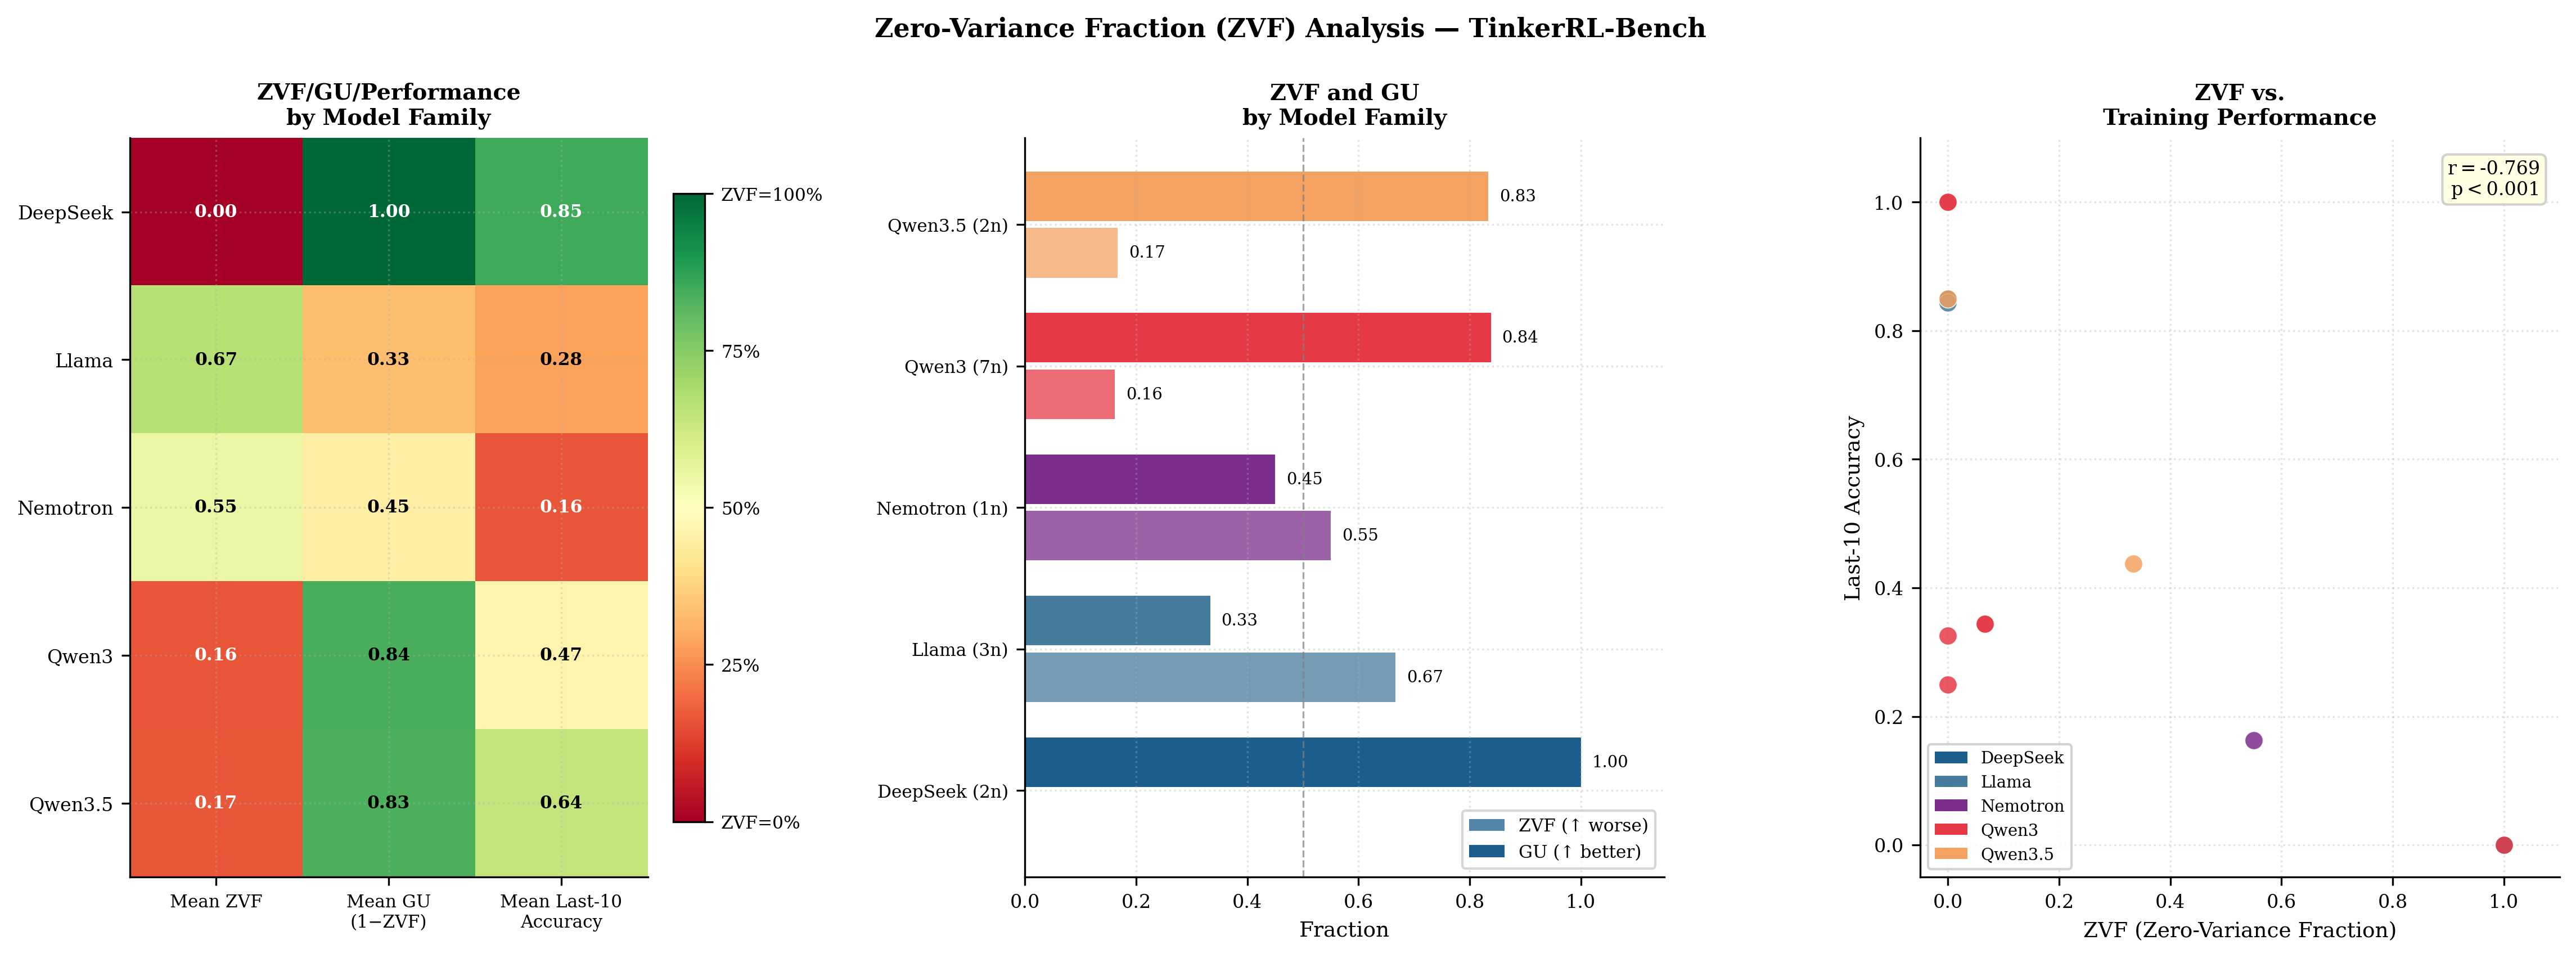
\includegraphics[width=\textwidth]{figures/v2/zvf_heatmap}
\caption{Per-step ZVF heatmap. Red: ZVF$=1$ (zero centered reward contrast);
blue: ZVF$=0$ (mixed rewards observed); grey: no data. Experiments sorted by
aggregate ZVF (descending).}
\label{fig:zvf-heatmap}
\end{figure}



% ---------------------------------------------------------------------------
\subsection{Connection to Contrastive Objectives and Group-Size Tradeoffs}
\label{sec:grpo-dpo}
% ---------------------------------------------------------------------------

GRPO and DPO admit related contrastive-gradient representations under specified
assumptions~\citep{wu2025grpodpo}, but differ in weighting and regularization.
Changing group size can change the expected update as well as its variance.
External efficiency observations do not establish a saving in this corpus.

\paragraph{ZVF Theory.}
\label{sec:zvf-theory}
For binary rewards, let $p_{q,t}$ be the success probability for prompt $q$.
With conditionally independent completions and equal prompt weights,
\begin{align}
\widehat{\mathrm{ZVF}}_t &= \frac1{m_t}\sum_{q=1}^{m_t}
 \mathbf{1}\{\widehat{\operatorname{Var}}(r_{q,1:G})=0\},\\
\mathbb E[\widehat{\mathrm{ZVF}}_t\mid p_{1:m_t,t}]
 &=\frac1{m_t}\sum_{q=1}^{m_t}h_G(p_{q,t}),\quad
 h_G(p)=p^G+(1-p)^G.
\end{align}
For $G>1$, $h_G$ is symmetric and U-shaped, not monotone over $[0,1]$.
At $G=2$, $1-h_2(p)=2p(1-p)$ is twice the Bernoulli variance.
In general the prompt average of $h_G(p)$ is not $h_G(\bar p)$.
At $G=8$, half the prompts at $p=0$ and half at $p=1$ give mean reward
$0.5$ and expected ZVF $1$; all prompts at $p=0.5$ have the same mean reward
and expected ZVF $1/128$. Increasing $G$ from 8 to 16 at $p=0.2$ increases
expected GU by approximately 13.96 percentage points, so diminishing returns
beyond eight completions are not uniformly negligible.

\paragraph{Descriptive theory comparison.}
The historical residual analysis used ten traces and a global mean reward.
Because prompt heterogeneity and completion dependence are not identified,
those residuals cannot diagnose adaptive sampling or correlated failures.
The binary model is an assumption-dependent reference, not empirical validation.
For a fixed $p$, reducing group size lowers the mixed-group probability; it
does not preserve all centered reward contrast.

\paragraph{Group-size display quarantine.}
The historical group-size panel pooled \texttt{campaign\_v2\_w2\_*},
\texttt{campaign\_v2\_w1\_qwen3-8b-base}, and
\texttt{scale\_gsm8k\_qwen3-8b} at $G=8$. It is not the same cohort as the
single-seed sweep in Table~\ref{tab:main_results}. Its apparent $G=4$
maximum is not an identified optimum, and the panel is excluded from this
root rather than presented as an interchangeable controlled ablation.


% ---------------------------------------------------------------------------
\subsection{Auxiliary Tool-Call Schema Compliance}
\label{sec:tool_use_cross_arch}
% ---------------------------------------------------------------------------

Tool-use is increasingly important for practical LLM deployments. We include
auxiliary tool-use probes to test schema-compliance reward environments across
model families.
Table~\ref{tab:tool_use_cross_arch} reports function-calling schema score
(fraction of calls with correct function name and valid argument schema).

\begin{table}[htbp]
\centering
\caption{Cross-architecture tool-call schema compliance on a post-training evaluation set. Schema compliance measures whether the model produces valid JSON with correct argument types under an evaluation schema-scoring protocol, not online RL reward or executed tool success. ``---'' entries either failed due to JWT authentication expiry or scored 0\% (task too difficult for the model).}
\label{tab:tool_use_cross_arch}
\small
\begin{tabular}{@{}lcccc@{}}
\toprule
\textbf{Family} & \textbf{Model} & \textbf{Base} & \textbf{Post-GRPO} & \textbf{Schema} \\
\midrule
Qwen3 & Qwen3-8B & 52\% & 70--71\% & 97\%$\to$100\% \\
Qwen3.5 & Qwen3.5-4B & \multicolumn{3}{c}{\textit{Not evaluated (training interrupted)}} \\
Llama-3.x & Llama-3.1-8B-Instruct & N/A & Functional & $\sim$100\% \\
DeepSeek & DeepSeek-V3.1 & \multicolumn{3}{c}{\textit{Not evaluated (training interrupted)}} \\
\midrule
\textit{Reference (prior work)} & Qwen2-0.5B & N/A & Functional & $\sim$100\% \\
\bottomrule
\end{tabular}
\end{table}

\paragraph{BrowserGym smoke result.}
After the main tool-use experiments, we also connected the Tinker/Atropos
training loop to BrowserGym MiniWoB through a real Chromium/Playwright browser
environment.  This smoke run is deliberately treated as systems evidence, not
as a benchmark result: it verified that prompts, browser observations, rollout
tables, W\&B logging, and Tinker checkpointing all route through the same
pipeline, but the one-step run obtained 0.0 reward and produced zero trainable
datum groups.  The archived rollouts show the key failure mode: the policy was
asked to emit actions over BrowserGym element ids, but the text-only
observation did not expose enough grounded DOM/accessibility detail, so the
model guessed ids rather than acting from observed affordances.  We therefore
separate browser-control integration from learned browser competence in
Table~\ref{tab:agentic_levels}.

\begin{table}[htbp]
\centering
\caption{Agentic evidence levels in this study. BrowserGym/MiniWoB is included
as an integration smoke test, not as learning evidence.}
\label{tab:agentic_levels}
\small
\begin{tabular}{@{}p{3.2cm}p{4.1cm}p{5.0cm}@{}}
\toprule
\textbf{Level} & \textbf{Evidence in this work} & \textbf{Interpretation} \\
\midrule
JSON/schema validity & SFT-warmed tool pipelines & Structured-output refinement after a behavioral prior exists.\\
Tool-name / argument shape & Custom tool-use rewards & Proxy for tool choice; argument values and execution are not fully verified.\\
Browser action routing & BrowserGym MiniWoB smoke & Tinker/Atropos/Chromium/W\&B integration works; reward remained 0.0.\\
Environment task success & Not yet established & Requires a MiniWoB/WebArena suite with grounded observations and baselines.\\
\bottomrule
\end{tabular}
\end{table}

% =============================================================================
% Experiment outcome footnotes (referenced from tables above)
% =============================================================================
\paragraph{Table footnotes.}
\begin{itemize}
    \item[$^\dagger$] Training interrupted before planned step count (partial run).
    Affected experiments:
    \texttt{scale\_gsm8k\_qwen3.5-27b} (10 steps), \texttt{scale\_gsm8k\_qwen3-32b} (10 steps),
    \texttt{frontier\_gsm8k\_qwen3-235b} (15 steps), \texttt{frontier\_gsm8k\_nemotron-120b} (20 steps),
    \texttt{moe\_gsm8k\_qwen3-30b-moe} (partial), \texttt{moe\_gsm8k\_qwen3-30b-inst} (partial).
    Additionally, \texttt{arch\_gsm8k\_gpt-oss-20b} did not produce usable data and is excluded
    from all tables. \texttt{arch\_gsm8k\_kimi-k2} completed (20 steps; peak 100\%, last-10 80.0\%)
    and is included in Table~\ref{tab:main_results}.
    \item[$^b$] DeepSeek-V3.1 GSM8K: 20 training steps on Tinker API;
    peak reward = 100\%, last-10 mean = 85.0\%, first-5 mean = 85.0\%.
    \item[$^h$] Direct KL divergence tracking failed due to PyTorch gradient graph error;
    reward-trajectory stability proxies (SI, PTD, Rolling Variance) are used
    instead---see Section~\ref{sec:kl} for the full proxy analysis.
\end{itemize}

% =============================================================================
\subsection{Campaign Extension: Additional Runs Under the Training-Reward Parser}
\label{sec:bitter_lesson}
% =============================================================================

We launched a systematic extension of 32 additional Tinker GRPO experiments
plus 3 TRL-GRPO stack-comparison experiments on Modal H100s, bringing our
total to 70+ training runs.  These runs are \emph{not} a test of the ``bitter
lesson'' hypothesis: they measure training-time reward under our existing
parsers, not held-out benchmark ceiling.  We keep them here for the ZVF/GU diagnostic
coverage they provide.

\paragraph{New Larger Models (training-reward parser, not held-out benchmark).}
We evaluated six previously untested models on GSM8K with GRPO (Table~\ref{tab:main_results}, Campaign Extension block).
\textbf{Kimi-K2-Thinking} had the highest sustained online reward in this block
(peak 100\%, last-10 95.8\%), suggesting that models already specialized for
reasoning may be better matched to this verifier-reward setup.
\textbf{Qwen3.5-397B-A17B}---the largest MoE model in our study at 397B total /
17B active---reached 100\% peak with 97.9\% last-10 average under
the training parser; this is an online-reward ceiling in the recorded campaign,
not a held-out benchmark ceiling. \textbf{GPT-OSS-120B} showed stable online
reward (93.8\% at step 1, 87.5\% last-10), consistent with reinforcement of an
already strong GSM8K prior rather than newly established capability. Conversely,
\textbf{DeepSeek-V3.1-Base} (671B/37B active) achieved only 57.3\% last-10
despite its scale, reinforcing that parameter count alone does not specify the
effective starting policy.

\paragraph{Stack Sensitivity, Not Framework Ranking.}
The TRL-GRPO experiments on Modal H100 expose a reporting problem rather than
a clean causal framework effect.  Under nominally matched visible
hyperparameters on Qwen3-8B, the Tinker row reaches 84.4\% last-10 reward while the TRL row reaches
5.0\% (peak 37.5\%).  This large divergence does not prove that Tinker is
better than TRL, because framework, backend defaults, sampler behavior,
loss masking, KL/reference handling, optimizer defaults, LoRA targets, precision/backend,
and evaluator details remain entangled.  It proves the more defensible point:
the phrase ``same GRPO config'' is under-specified unless those hidden stack
variables are logged and controlled.  The Llama-3.1-8B-Instruct row performs
substantially better (71.3\% last-10), reinforcing the stack-conditioned
interpretation rather than a universal framework ranking.

\paragraph{Base vs.~Instruct Models.}
A clear pattern emerges: base models (Llama-3.1-70B at 36.4\%, Llama-3.1-8B at 11.5\%, DeepSeek-V3.1-Base at 57.3\%) struggle substantially compared to instruct counterparts (qualitative, no statistical test).
This aligns with the GRPO-as-DPO interpretation~\cite{wu2025grpodpo}: GRPO requires models that already produce \emph{some} correct completions to generate meaningful preference pairs.
Base models lacking instruction-following capability produce uniformly low-quality completions, yielding zero-variance groups that prevent learning.

\paragraph{Group Size Ablation.}
We swept group size $G \in \{2, 4, 8, 16\}$ on Qwen3-8B (Table~\ref{tab:main_results}, Group Size block).
The highest observed last-10 reward in this single-seed 30-step sweep occurs at
$G{=}8$ (84.4\%), with $G{=}4$ second (52.1\%) and both $G{=}2$ (37.5\%) and
$G{=}16$ (38.0\%) lower. This inverted-U pattern is consistent with a finite-group
tradeoff: too few samples can miss reward diversity, while larger groups can
increase rollout cost and change the effective update distribution. A completed
multi-seed sweep would be needed before calling $G{=}8$ optimal.

% =============================================================================
\section{Reproducibility}
\paragraph{Figure provenance boundary.}
Checked-in figure assets are historical snapshots. A successful TeX build does
not validate their data selection, task labels or metric definitions. Before
submission, every consumed figure must bind a source snapshot, generator
revision, metric/cohort specification and output hash in a clean rebuild.
The existing v2 assets are not certified by this source-only correction.

\label{sec:reproducibility}
% =============================================================================

Reproduction is partial, not guaranteed by a fixed seed or a Docker image.
Table~\ref{tab:availability-audit} separates local implementation, backend
configuration, and accessible evidence. W\&B is run-level metadata unless a
named export establishes step traces. Failed direct-KL logging does not become
available merely because corrected code exists. Private mirrors and account
names are not public checkpoint releases; wildcard URLs are not immutable
checkpoint identifiers. No claim that all checkpoints or all logs are public
is made. Each future release needs exact artifact URLs, revisions, access
requirements, and hashes before it is treated as independently reconstructible.

\begin{table}[htbp]
\centering\small
\caption{Implementation and evidence availability by scope.}
\label{tab:availability-audit}
\begin{tabular}{p{.28\linewidth}p{.62\linewidth}}
\toprule
Scope & Availability and boundary \\
\midrule
Local runner & Reward processing and custom loss inspectable in source; version-specific \\
Managed configuration & Requested hyperparameters inspectable; execution identity requires logs \\
Server internals & Hardware placement, scheduling, and backend numerics undisclosed \\
Reviewed tool-use cells & Descriptive manuscript observations; held-out not evaluated \\
Historical traces & Local logs may exist; public completeness and exact run mapping unresolved \\
W\&B / checkpoints & Credentials or revision-specific verification may be needed \\
Direct KL & Failed telemetry in affected runs; no recovered trace claimed \\
\bottomrule
\end{tabular}
\end{table}


% =============================================================================
% =============================================================================


\section*{Trust Calibration and Empirical Scope}
To ensure transparency, we explicitly calibrate the claims of this report against the underlying evidence:
\begin{itemize}
    \item \textbf{Noncanonical Runner:} Our training loop is a noncanonical group-relative policy-gradient runner, not a faithful GRPO reproduction (it omits PPO ratios, clipping, and reference-KL penalties).
    \item \textbf{Statistical Power:} All $p$-values and effect sizes reported for training traces are exploratory diagnostics over autocorrelated steps, not confirmatory tests over independent replicates, as most Tinker runs are single-seed.
    \item \textbf{Proxy Rewards:} Our tool-use and code generation rewards evaluate schema compliance and restricted-sandbox parsing, respectively, rather than end-to-end semantic capability.
    \item \textbf{Confounding Factors:} Any observed architectural differences (e.g., dense vs. MoE) or scaling patterns are confounded by initialization and framework choices, serving as hypothesis generation rather than causal proof.
    \item \textbf{Reproducibility:} While we provide extensive local artifacts, full independent reconstruction is partial due to our reliance on opaque external backends.
\end{itemize}

% ---------------------------------------------------------------------------
\subsection{Prospective hypotheses when ZVF persists}
\label{sec:zvf_intervention}

The ZVF/GU diagnostic identifies regimes, but it does not identify a remedy.
The following are related or prospective hypotheses, not interventions supported
by the reviewed record. Any comparison requires a predeclared, matched-budget
evaluation with held-out outcomes.

\paragraph{Hypothesis 1: a $G=2$ comparison.}
Wu et al.~\citep{wu2025grpodpo} relate contrastive representations, not universal
GRPO--DPO equivalence. For conditionally iid binary completions at a fixed
prompt, expected GU at $G=2$ is $2p(1-p)$, twice the Bernoulli variance.
A comparison must match a declared resource budget and held-out endpoint.

\paragraph{Hypothesis 2: resampling or warm-start.}
Resampling and warm-start SFT are prospective arms. The two reviewed all-wrong
cells do not establish why their rewards were homogeneous or which remedy helps.
Any effect on held-out outcomes must be evaluated under matched budgets.

\paragraph{Hypothesis 3: a TPO-style objective.}
TPO~\citep{kaddour2026tpo} constructs $q\propto p_{\mathrm{old}}\exp(u/\eta)$.
For homogeneous rewards, $u=0$ and $q=p_{\mathrm{old}}$. At the rollout snapshot
$p_\theta=q$, so the first-epoch grouped reward-directed gradient is zero.
Later reuse after informative updates can anchor the policy. Its benefit here
remains a prospective matched-budget question, not a five-step recommendation.

% =============================================================================
% =============================================================================


\section*{Claims We Explicitly Do Not Make}
\label{sec:claims_we_do_not_make}

This paper is an engineering diagnostic, not a benchmark result, not a new algorithm, and not a clean causal study. The runner is GRPO-style but omits the PPO ratio/clip, the frozen reference policy, and the completion-only token mask; the HumanEval-style sandbox strips Python built-ins; the tool-use reward scores JSON schema rather than tool execution; and most Tinker runs are single-seed on a 30-step horizon. PPO/GRPO comparisons are backend-, sampler-, optimizer-, LoRA-, and checkpoint-confounded. The historical selected-checkpoint aggregate is withdrawn rather than compared with the reviewed record. Readers should treat the manuscript as a candid engineering audit whose narrow defensible contribution is reward-diversity triage (ZVF/GU) plus stack-identifiability reporting discipline, not a leaderboard or algorithm paper.

To bound the attack surface of this empirical study, we explicitly disclaim the following:

\begin{itemize}
    \item We do not claim canonical GRPO superiority or that this runner represents canonical GRPO.
    \item We do not claim broad reasoning improvement across tasks or model families.
    \item We do not claim tool-execution competence; tool-call results measure schema compliance only.
    \item We do not claim generalization from test-split reward probes (MATH-500, HumanEval training pools).
    \item We do not claim frontier scaling laws from short, noisy training traces.
    \item We do not claim PPO-vs-GRPO algorithm superiority rankings.
    \item We do not claim GRPO universally improves reasoning or achieves state-of-the-art GSM8K/MATH performance. The later, separate five-seed Qwen3-8B held-out comparison is not reviewed-record evidence: $82.0\% \to 83.3\%$ has $p=0.26$ from a one-sample seed-level test against a fixed baseline, not a paired-seed test.
    \item We do not claim ZVF predicts final performance. ZVF is a triage diagnostic that identifies training regimes (cold-start collapse vs. saturation vs. healthy contrast); it is not a calibrated performance predictor. The zero-order correlation ($r = -0.769$) is largely confounded by current reward level on binary tasks; the partial correlation controlling for $R_t$ at lag 5 is only $r = 0.059$ (descriptive only; no calibrated p-value).
    \item We do not claim group size $G=8$ is globally optimal. The group-size ablation was single-seed and 30-step; multi-seed validation is needed before calling $G=8$ optimal.
    \item We do not claim Dense models outperform MoE architectures at matched active parameters. The Dense vs MoE comparison is confounded by base vs instruct initialization; the architecture effect cannot be isolated from the initialization effect.
    \item We do not claim significant cross-library performance variance. We demonstrate substantial cross-library divergence under nominally matched configurations; the single-seed Tinker runs lack variance estimates and do not support significance claims.
\end{itemize}

\section*{What We Do Claim}
\label{sec:what_we_claim}

The contribution list is the same as in the abstract and introduction:
(i) the specified runner's centered reward-contrast identity;
(ii) an evidence audit with descriptive cells and unresolved-cohort quarantines;
and (iii) a reporting and prospective operator-evaluation contract.
The identity is elementary and no priority for the ZVF definition is claimed.
Historical auxiliary results below and above are context, not additional
validated claims. The associated thesis Table~6.2 remains provisional; this
audit does not change its numbers or upgrade its status.

\section{Limitations}
\label{sec:limitations}
% =============================================================================

This section defines the evidentiary boundary for the claims.  The paper's
central contribution is the diagnostic one: in a critic-free group-relative RL
loop with binary or verifier-like rewards, within-group reward diversity
determines whether the update has usable signal.  ZVF/GU are therefore proposed
as early triage measurements, not as proof of broad reasoning improvement, not
as an algorithm diagnostic baseline, and not as a replacement for held-out evaluation.
The limitations below state which claims are constrained and which claim remains
supported.

% -----------------------------------------------------------------------
\subsection{Infrastructure and Observability Limits}
\label{sec:infra_failures}
% -----------------------------------------------------------------------

\paragraph{Managed-backend interruptions.}
Several managed-backend jobs stopped before their planned horizon because of
credential expiry or wall-clock limits.  We do not impute missing steps or
compare interrupted rows against completed rows as if they were equivalent:
partial runs are marked $\dagger$ and used only for observed-step telemetry;
most managed runs are short-horizon and single-seed.
This weakens scale and convergence conclusions.  It does not by itself weaken
ZVF/GU measurements computed on completed logged steps, because those diagnostics
only require the sampled group rewards at the steps being analysed.

\paragraph{Closed-source and backend-specific implementation.}
Tinker is a managed, closed-source training service.  We cannot audit its exact
loss implementation, sampler, minibatch construction, normalization details,
precision stack, scheduler, or hardware placement.  Accordingly, Tinker rows are
measurements of a \emph{realized managed stack}, not measurements of canonical
GRPO as a mathematical object.  Any comparison such as ``PPO versus GRPO'' is
therefore stack-conditioned unless the backend, model checkpoint, prompt
template, sampler, loss mask, KL/reference handling, LoRA configuration,
optimizer, checkpoint rule, and evaluator are held fixed or explicitly modeled.

\paragraph{Telemetry gaps.}
Direct KL tracking failed in the affected runs, and the W\&B API export does
not contain reliable step-level reward time series for all experiments.  The
step-level plots and ZVF/GU analyses therefore rely on local CSV/checkpoint
logs, while W\&B should be treated as run-level metadata unless a row states
otherwise.  Stability Index, Peak-to-Tail Drift, and Rolling Variance are
symptom-level indicators; they are not measurements of per-token
KL.  This limits policy-drift claims, but it is separate from the ZVF/GU claim,
which is computed directly from reward equality within sampled groups.

% -----------------------------------------------------------------------
\subsection{Methodological and Statistical Scope}
\label{sec:method_limits}
% -----------------------------------------------------------------------

\paragraph{A GRPO-style runner, not canonical GRPO.}
The main training runner preserves the critic-free, group-normalized-advantage
structure needed for the ZVF/GU analysis, but it omits several elements often
associated with canonical implementations: a PPO probability ratio and clipping
term, a frozen reference-policy KL penalty, and a completion-only token mask in
some runs.  Therefore the paper's safest algorithmic claim is about a
\emph{group-relative critic-free RL loop under the reported stack}, not about all
possible GRPO implementations.

\paragraph{Short horizons and limited replication.}
Most managed experiments use short horizons and single seeds, primarily because
frontier-scale managed training is expensive and failure-prone.  These runs are
suitable for studying early learning-signal availability, collapse, saturation,
and stack sensitivity.  They are not sufficient for asymptotic convergence,
state-of-the-art performance, long-horizon reward hacking, or robust algorithm
ranking.  Where multi-seed or held-out analyses exist, they are reported
separately; otherwise numbers should be read descriptively, consistent with the
replication cautions of \citet{henderson2018deep}
and~\citet{jordan2024benchmarking} regarding the limits of
single-platform papers.

\paragraph{Held-out capability evidence is narrow.}
The later, separate five-seed GSM8K 200-example comparison reports $82.0\%$ to
$83.3\%$. Its $p=0.26$ is a one-sample seed-level test against the fixed
baseline, not a paired-seed test, and it is not reviewed-record evidence.
Consequently, the paper does not claim a significant held-out math improvement.
Training rewards support statements about optimization dynamics
inside a particular reward environment; they do not establish general reasoning,
code, or tool-use capability.

\paragraph{Public benchmark and contamination risk.}
GSM8K, MATH-style prompts, and HumanEval are public benchmarks, and we cannot
rule out that base models saw related examples during pretraining or instruction
tuning.  The held-out split is held out from \emph{our fine-tuning loop}, not
from the upstream training histories of the base models.  Absolute performance
therefore should not be interpreted as novelty on unseen tasks; the defensible
comparison is relative to each run's initialization and logged reward
environment.

\paragraph{Missing competitive baselines.}
The study does not exhaust strong alternatives such as SFT-only warm-starts,
bestof-$N$ sampling, rejection sampling, DAPO/Dr.~GRPO-style corrections, or
longer-budget PPO/GRPO variants under fully matched infrastructure.  This is a
limitation for performance claims.  It is less damaging to the paper's main
diagnostic contribution, because ZVF/GU ask whether the sampled reward groups
contain contrast, not which optimizer exploits it.

% ---------------------------------------------------------------------------
\subsection{Reward-Proxy and Length-Bias Risks}
\label{sec:length_bias}
% ---------------------------------------------------------------------------

\paragraph{Proxy rewards.}
Several environments intentionally measure proxies.  The Tinker tool-use rows
score schema/function-call form rather than executed tool success; the
HumanEval-style sandbox removes Python built-ins such as \texttt{len},
\texttt{range}, and \texttt{sum}; and the MATH reward mixes final-answer matching
with \texttt{\textbackslash boxed\{\}} formatting.  The MATH-500 and HumanEval
prompt pools used in the training loop are reward-environment probes rather
than held-out generalization tests.  These rows are useful for studying whether
the rewarder supplies contrast, but they should not be upgraded into broad code,
math, or tool-use claims.

\paragraph{Length bias and reward hacking are not fully measured.}
Prior work shows that GRPO-like objectives can be sensitive to length bias and
verbosity-trap dynamics~\citep{tong2025drgrpo}.  Our telemetry
flags peak-to-tail reward regressions and verbosity-trap-like trajectories, but
we do not uniformly log response length, direct KL, or long-horizon behavior
across all runs.  Thus the current data can show reward instability and motivate
length-normalized objectives; it cannot prove that length alone caused the
observed regressions.  Dr.~GRPO, length penalties, and sequence-normalized
objectives remain untested mitigations in this artifact.

\paragraph{Net effect on the paper's claims.}
These limitations remove broad performance claims and universal algorithm
rankings.  What remains is deliberately narrower: ZVF/GU give a practical way to
ask whether a verifier-style reward is producing the within-group contrast that
a critic-free group-relative update needs.  The paper's contribution is strongest
when read as a diagnostic and reporting framework for RL post-training
stacks, not as evidence that this runner generally improves model capability.

% =============================================================================
\subsection{Broader Impact}
\label{sec:impact}
% =============================================================================

\paragraph{Alignment and Misuse.}
GRPO and related RLHF methods are dual-use technologies. On the positive side,
they are the primary mechanism by which frontier models are aligned to human
preferences, and our audit artifact lowers the barrier to studying these methods
rigorously. On the negative side, the same reward-maximization machinery can
be directed at adversarial objectives---optimizing for reward-hack proxies,
generating persuasive misinformation, or circumventing safety classifiers. We
do not provide new attack capabilities, but improvements in RL post-training
efficiency reduce the compute budget required for such misuse. We encourage
the community to develop robust reward modeling and out-of-distribution
detection in parallel with efficiency advances.

\paragraph{Democratizing RL-for-LLM Research.}
A primary motivation for \ours{} is to make rigorous RL post-training
experiments accessible to researchers without large-scale compute. By
publishing standardized tasks, Docker containers, and cost-annotated run
logs, we aim to reduce the advantage that well-resourced labs hold in this
space. Our total experimental expenditure was modest: approximately \$120 in
Tinker API credits (including unsuccessful or interrupted attempts),
and roughly \$95 in Modal compute for the six held-out evaluation jobs
(three of which timed out). Open-source backend experiments were conducted on
a single A100 node donated by PES University's LLM Research Group. We include
these cost breakdowns explicitly so that other groups can budget accordingly.

\paragraph{Training Data and Privacy.}
All training data is drawn from publicly released datasets: GSM8K
\citep{cobbe2021training} for mathematical reasoning, HumanEval
\citep{chen2021codex} for code generation, and a synthetic tool-use corpus
generated without human subjects. No private data, personally identifiable
information, or licensed proprietary content is used. The audit corpus does not
involve human participants in any capacity, and no IRB review was required.

\paragraph{Limited incremental dual-use risk.}
Our contribution is a \emph{diagnostic audit framework}, not a new model or capability. We do not release any model trained on sensitive, harmful, or restricted content. Evaluated checkpoints derive from publicly available base models under their respective licenses: Qwen model families under Apache-2.0; Llama-3.x model families under Meta's Llama Community License; DeepSeek-V3.1 and Nemotron under their respective community/commercial terms. We do not claim all bases are Apache/MIT-equivalent. We do not introduce a new hazardous dataset or attack method, but improved RL post-training workflows are dual-use in the general sense that any optimization advance can lower cost for misuse; we discuss this as a qualitative residual risk rather than claiming no direct risk.

\paragraph{Reproducibility Statement.}
Despite the infrastructure failures documented above, all successfully
completed experiments are reproducible via Docker containers, fixed random
seeds, and step-by-step commands in \texttt{REPRODUCE.md}. Corrected logging
and KL-tracking code is included in the release. We have archived all local
CSV training logs so that the step-level reward trajectories excluded from
W\&B are nonetheless available to other researchers.

% =============================================================================
\subsection{Discussion}
\label{sec:discussion}

\subsection{Why Might Stack-Conditioned Algorithm Effects Vary?}
\label{sec:discuss_model_algo}

The sharpest observation in our audit corpus is not a stable algorithm ranking,
but the fact that such a ranking is not identifiable from the available
artifacts.  The Qwen PPO/GRPO row changes interpretation depending on which
result summary is treated as canonical, while PPO is substantially higher in
the recorded Llama-3.1-8B setting (strong descriptive rank correlation on
per-step rewards).  However, these rows are single-seed and backend-confounded,
and the Mann-Whitney $p$-value assumes independent observations while per-step
rewards within a single trajectory are
autocorrelated.  We present three mechanistic hypotheses that future work
can test with proper multi-seed replication.

\paragraph{Hypothesis 1: Reward landscape geometry.}
GRPO replaces the value-function baseline of PPO with a within-group reward
mean, computing advantages purely from peer comparisons.
This estimator is low-variance when the per-prompt reward surface is smooth
enough that sampled completions span a reliable gradient direction --- a
condition more likely to hold when the model's prior task performance exceeds a
threshold (roughly 80--90\% on comparable tasks).
Qwen3-8B enters GSM8K training with a high zero-shot baseline, providing a
reward landscape that is largely flat with narrow high-reward ridges.  This
setting may favor group-relative contrast in some stacks, but the current
artifacts are not clean enough to make that a directional algorithm claim.
Llama-3.1-8B enters at a lower zero-shot baseline, presenting a rougher
landscape where the value function's global smoothing is beneficial.
This conjecture predicts that, under similar verifier-reward and sampling
conditions, group-relative methods may be more competitive when the model
already samples some correct completions, whereas value-function methods may
help when the initial reward landscape is rougher. Our data are too small and
confounded to support a prescriptive GRPO-vs-PPO rule.

\paragraph{Hypothesis 2: Instruction-tuning quality modulates advantage noise.}
Both Qwen3-8B and Llama-3.1-8B are instruction-tuned, but they differ in
instruction-following fidelity and output format consistency.
Inconsistent formatting inflates the within-group reward variance for reasons
unrelated to mathematical reasoning quality, injecting noise into GRPO's
advantage signal.
PPO's value function, trained jointly on the task, can absorb some of this
format-related variance and focus the policy gradient on reasoning-relevant
features.
This hypothesis is consistent with our MoE finding: the base (non-instruct)
Qwen3-30B-A3B achieves only 50\% peak GRPO reward, while the instruction-tuned
variant reaches 100\% --- the initialization quality effect is substantial and
independent of architecture.

\paragraph{Hypothesis 3: Reference-policy proximity.}
Canonical GRPO includes a reference-policy KL term~\citep{shao2024deepseekmath}.
The audited runner omits it. Reward levels, ZVF, and SI do not identify KL or
proximity to initialization. A proximity hypothesis needs direct token-level
distribution measurements under a specified reference, not reward proxies.

\paragraph{Mechanism checks and prospective operator benefit.}
Hold policy, sampled completions, and token masks fixed and intervene on reward
vectors to verify centered coefficients and their reward-gradient contribution.
This is distinct from randomizing prospective sampling policies over a common
task population, matching budgets, and evaluating held-out outcomes.
Stratifying different prompts changes content and difficulty as well as rewards.
At $G=8$, $h_8(0.2)=h_8(0.8)\simeq0.168$ and $h_8(0.25)\simeq0.100$;
25\%/75\% cutoffs do not define near-degenerate groups. Define such a regime
through a prespecified target $h_G(p)$ with estimation uncertainty.
Freeze any diagnostic rule, define its endpoint independently, compare nonlinear
reward/history baselines, and hold out entire runs or tasks. A lower ZVF alone
is not operator benefit.

\paragraph{Prespecified evaluation of a diagnostic policy (future work).}
Compare continuing the fixed schedule, a declared dynamic-sampling/retry rule,
and the proposed diagnostic policy using common initializations, tasks,
evaluators, and a fixed generation budget. Charge discarded and resampled
completions, token lengths, and any warm-start training to that budget.
Measure held-out quality at budget exhaustion, expenditure, false stops, and
recovery; include all-failure groups with correct and malformed verifiers,
all-success groups, mixed groups without improvement, and initially
unproductive runs that later recover. Compare flexible reward mean/slope/history
baselines with all-wrong/all-correct fractions, success-count distributions,
and advantage variance before attributing incremental value to ZVF.
Independent training seeds are the replication unit; sample size follows a
prespecified effect or precision target and adequate failure-event coverage,
not a rule that five seeds guarantees validation. No such prospective result
is reported here.


\subsection{What Stack Sensitivity Means for the Field}
\label{sec:discuss_impl}

The classical RL-library rows (SB3, CleanRL, Tianshou) are useful engineering
sanity checks, but they are not evidence for a framework ranking in LLM
post-training.  Their near-random arithmetic performance primarily shows that
a text-generation policy cannot be treated as a standard continuous-control
MDP without explicitly specifying tokenization, autoregressive rollout,
loss masking, reward parsing, and action construction.  This is stack
mis-specification evidence, not evidence that PPO-the-algorithm fails.

The practical implication is narrower and stronger: published comparisons
such as ``PPO versus GRPO'' are underidentified unless the realized treatment
is specified.  A defensible comparison must state the model checkpoint and
tokenizer, prompt template, reward parser, sampler and grouping process, loss
mask, KL/reference handling, optimizer, LoRA targets, precision/backend, and
evaluator.  Without those details, an algorithm label is not enough to tell
whether two rows are comparable.

\subsection{Connections to Concurrent Work}
\label{sec:discuss_related}

\paragraph{AERO and ZVF as a training diagnostic.}
\citet{zhang2026aero} motivate AERO by the prevalence of zero-advantage dead
zones in GRPO training and propose a Bayesian posterior over prompt difficulty
to pre-screen prompts.
Our ZVF measurement ($r = -0.769$, $p < 0.001$ with final performance) provides
an empirical calibration point for the phenomenon AERO targets, while the
lagged analysis in Section~\ref{sec:zvf-lagged} keeps the claim scoped:
ZVF is useful for triage, not as a standalone performance predictor.
Importantly, our data reveal a critical boundary condition: ZVF is \emph{task-driven, not model-scale-driven}:
tool-use experiments saturate at $\text{ZVF} = 100\%$ regardless of model size,
while GSM8K experiments average $\text{ZVF} = 8.5\%$ across the same model
range.
This suggests that AERO's compute savings will be largest when the task is
poorly matched to the model's prior capabilities --- precisely the
regime where standard GRPO training is most wasteful.
Our ZVF measurements can serve as a calibration dataset for AERO's Beta prior.

\paragraph{Descriptive saturation fits and their limits.}
\citet{nimmaturi2025scalinglaws} derive a three-phase exponential saturation
law for GRPO, finding that 80\% of training steps contribute marginally and
proposing early stopping.
We observe a compatible three-phase pattern in 73\% of LLM fine-tuning
experiments, while treating it as descriptive because the traces are short.
However, our data reveal a critical boundary condition: the saturation
framework \emph{fails for unstable training runs}.
Nemotron-120B's trajectory (87.5\% peak $\to$ 16.2\% last-10) is
non-monotonic and cannot be fit by the exponential saturation model ---
it is better characterized as a reward excursion followed by policy
collapse, a regime the scaling law does not model.
We recommend that practitioners verify monotonicity before applying early
stopping rules derived from the saturation model.

\paragraph{Contrastive objectives and TPO are distinct.}
Wu et al.~\citep{wu2025grpodpo} analyze GRPO--DPO connections with weighting
and regularization qualifications. TPO~\citep{kaddour2026tpo} is a separate
objective; its homogeneous-group first-epoch gradient is zero at the rollout
snapshot, as discussed in Section~\ref{sec:zvf_intervention}. Neither work
validates a five-step intervention rule for this audit.

\subsection{Limitations of Proxy Metrics and the Path to Direct KL Measurement}
\label{sec:discuss_kl}

Our reward-instability analysis relies on three reward-trajectory proxies (SI, PTD,
Rolling Variance) that are associated with late reward in this artifact
($r = -0.517$, $p = 0.005$ for PTD, uncorrected) but are not the same as direct
KL divergence measurements.
The proxies capture \emph{observable symptoms} of reward instability --- reward
instability and peak-to-tail degradation --- but cannot distinguish between
two importantly different causes: (a) the policy has genuinely drifted far from
the reference in token-distribution space, or (b) the reward function is
inherently noisy and the policy is stable but reward variance is high.
Nemotron-120B's collapse is almost certainly case (a), given that its reward
decline is monotonic and persistent; but for models with moderate PTD (0.1--0.3),
the two causes are indistinguishable from reward trajectories alone.

Corrected KL tracking code is released in \texttt{src/grpo\_trainer.py} and
should be validated on at least the two Modal runs (Qwen3-8B and
Llama-3.1-8B) where GPU access is reproducible.
Additionally, the per-token divergence framework of \citet{liu2025rlsubnetworks}
--- which measures which parameters actually update during RL fine-tuning ---
could reveal whether the small subnetwork they identify has higher KL per
parameter, potentially explaining why moderate-sized models sometimes exhibit reward collapse consistent with drift (rather than direct evidence of catastrophic drift, which would require direct KL or policy-distance telemetry we do not have) despite updating only 5--30\% of weights.
Connecting our behavioral proxy metrics to this parameter-level analysis is a
natural and important next step.
